\documentclass[a4paper,onecolumn,11pt]{quantumarticle}
\pdfoutput=1
\usepackage[utf8]{inputenc}
\usepackage[english]{babel}
\usepackage[T1]{fontenc}
\usepackage{amsmath}
\usepackage{amsfonts}
\usepackage{hyperref}
\usepackage{algorithm}
\usepackage{algpseudocode}
\usepackage{tikz}
\usepackage{lipsum}
\usepackage{graphicx}
\usepackage{subcaption}
\usepackage{physics}
\usepackage[normalem]{ulem}
\usepackage{color,soul}
\renewcommand{\arraystretch}{1.5}
\usepackage[normalem]{ulem}

\DeclareMathOperator*{\argmax}{argmax}
\algrenewcommand\algorithmicrequire{\textbf{Input:}}
\algrenewcommand\algorithmicensure{\textbf{Output:}}

\newtheorem{theorem}{Theorem}

\begin{document}

\title{Automated Quantum Circuit Design with Nested Monte Carlo Tree Search}

\author[1]{Peiyong Wang}
\orcid{0000-0002-0665-6639}
\email{peiyongw@student.unimelb.edu.au}

%\thanks{You can use the \texttt{\textbackslash{}email}, \texttt{\textbackslash{}homepage}, and \texttt{\textbackslash{}thanks} commands to add additional information for the preceding \texttt{\textbackslash{}author}. If applicable, this can also be used to indicate that a work has previously been published in conference proceedings.}


\author[2]{Muhammad Usman}
\orcid{0000-0003-3476-2348}

\author[1]{Udaya Parampalli}
\orcid{0000-0002-9798-0134}

\author[2]{Lloyd C. L. Hollenberg}
\orcid{0000-0001-7672-6965}

\author[1]{Casey R. Myers}
\orcid{0000-0002-8838-7523}

\affil[1]{School of Computing and Information Systems, Faculty of Engineering and Information Technology, The University of Melbourne, Melbourne VIC 3010, Australia}
\affil[2]{Centre for Quantum Computation and Communication Technology, School of Physics, The University of Melbourne, Parkville, VIC 3010, Australia}

\maketitle

\begin{abstract}


%In this article, we report a Monte-Carlo Tree Search (MCTS) based method for automated design of quantum circuits. By reformulating the searching problem in a tree structure and MCTS, our method can operate even when the search space is very large. Our algorithm achieved good \textcolor{red}{[need a stronger, more positive statement here: our results are better, or more competitive...]} performance on tasks like searching for different encoding circuits of the [[4,2,2]] quantum error detection code, the ansatz for finding the ground state energy of the hydrogen molecule $H_2$ as well as variational circuit that can find one of the solutions to a \textsc{MaxCut} problem. \textcolor{red}{[Fix the abstract last]}

Variational quantum algorithms are one of the most promising methods to construct quantum solutions and have found myriad applications in the last few years. Despite the adaptability and simplicity, their scalability and the selection of suitable ans\"atzs remain key challenges. In this work, we report an algorithmic framework based on nested Monte-Carlo Tree Search (MCTS) and combinatorial multi-armed bandit for the automated design of quantum circuits. Through numerical experiments, we demonstrated that our algorithm can be applied to various kinds of problems, including the ground energy problem in quantum chemistry, quantum optimization on a graph, solving  systems of linear equations, and finding encoding circuit for quantum error detection codes. Compared to the existing research in this area, our algorithm can explore larger search spaces and optimise quantum circuits for larger systems, showing both versatility and scalability.


\end{abstract}
%\tableofcontents
\section{Introduction}\label{intro}

%%%
% paragraph: introduce variational quantum circuits, and point out the difficulty to find a suitable ansatz
%%%
Variational quantum circuits, first proposed for solving the ground state energy problem for molecules \cite{peruzzo2014variational}, now underpin the solution to many open research problems including in the field of quantum machine learning \cite{schuldpetruccione2021}, quantum chemistry \cite{RevModPhys.92.015003}, option pricing \cite{2020optionpricing} and quantum error correction \cite{johnson2017qvector, Xu2021-dt}. However, choosing a suitable ans\"atz is not an easy task because generally the search space is very large and it is not well established whether there is a common principle for designing such ans\"atz. For problems involving physical systems such as in quantum chemistry, we can rely on the well-defined properties of molecular systems for ans\"atz designing, like the  hardware efficient ansatzes~\cite{2017hardwareefficientvqe} and physical-inspired ansatzes, such as $k$-UpCCGSD~ \cite{physicalinspiredansatze1doi:10.1021/acs.jctc.8b01004}. However, this cannot be generalised to other areas such as designing variational error correction circuits or quantum optimisation problems. For example, in \cite{Xu2021-dt}, when developing a variational circuit that can encode logical states for the 5-qubit quantum error correction code, the authors randomly searched over a large number (order of 10000) of circuits. It is anticipated that, with the increasing number of application areas for variational quantum circuits and the need for scalability to tackle large size of problems without good physical properties, such random search methods or methods based purely on human heuristics will struggle to find suitable ans\"atzes. Therefore, it is important to develop efficient methods for automated design of variational quantum circuits by leveraging the power of artificial intelligence (AI) which can be deployed for a wide range of applications.

\textcolor{red}{\textbf{Try to make a coherent story from paragraph 2 and 3 by combining them into just 1 small paragraph. The message should be that AI is a powerful tool to discover new knowledge by efficiently and systematically looking into very large search spaces which is directly relevant to your work... So you give this message in this paragraph and then use two or three examples to support your argument. }}

%%%
% a paragraph for AI for science. Starting from AlphaGo's move 37 when playing against Lee Sedol, which is beyond human intuition, followed by a few sentences on what could AI bring to scientific research
%%%
\textcolor{red}{The power of AI is not just restricted to areas like image and natural language processing, but it has also enabled discovery of new knowledge. In 2016, DeepMind's Go playing AI AlphaGo \cite{AlphaGoDBLP:journals/nature/SilverHMGSDSAPL16} defeated world champion Lee Sedol, with Move 37 in Match 2 surprising most professional Go players as creative and unique, also nearly impossible to be played by human players. Beside ingenuity of playing go, artificial intelligence algorithms also demonstrated vast potential in making scientific discovery. In 2020, DeepMind participated the 14th Critical Assessment of protein Structure Prediction (CASP) competition and, with a neural network based model called AlphaFold2, achieved competitive accuracy on predicting the three-dimensional structure of proteins solely based on the amino acid sequence, compared to the structures obtained by experiments. AlphaFold2 managed to discover new mechanism for the bonding region of the protein and inhibitors \cite{alphafold2Jumper2021-lw}. In 2021, AI scientists teamed up with mathematicians in the quest to discover new structures and patterns in topology and representation theory with the assistance of machine learning algorithms. The machine learning algorithm developed in \cite{Davies2021-xh} discovered some new relationships between geometric invariants and algebraic invariants in knot theory, as well as new insights in the combinatorial invariance conjecture, which is to calculate the Kazhdan-Lusztig polynomial of two elements in the symmetry group with their unlabeled Bruhat interval, which can be viewed as a directed graph.}


%%%
% paragraph: point out the similarity between deep neural networks and variational quantum circuits. especially the design of architectures. They both require to choose from a set of operations to compose a network/circuit.
%%%
\textcolor{red}{Like variational quantum circuits, modern deep neural networks also require to select from different kinds of operations when composing the neural network, like different convolution kernels or different skip connections. Such a design question is called Neural Architecture Search (NAS). Facing the similar design questions as variational quantum circuits, researchers in the area of artificial intelligence and deep learning have also seek to apply search algorithms to designing neural networks. Famous endeavors include the DARTS algorithm \cite{DARTS_DBLP:conf/iclr/LiuSY19}, which models the choice of operations placed in different layers as an independent categorical probabilistic model that can be optimized via gradient descent methods, and the PNAS algorithm \cite{PNAS10.1007/978-3-030-01246-5_2}, which models the search process with sequential model-based optimization (SMBO) strategy, as well as ENAS \cite{ENASpmlr-v80-pham18a}, which is the first and feasible neural architecture search algorithm that requires far less GPU hour than its predecessor and can finish within one day. Tree-based algorithms were also proposed for NAS, such as AlphaX \cite{AlphaXDBLP:conf/aaai/WangZJTF20}, which models the search process similarly as the search stage of AlphaGo \cite{AlphaGoDBLP:journals/nature/SilverHMGSDSAPL16}. Recently, a new NAS algorithm based on tree search and combinatorial multi-armed bandits, proposed in \cite{huang2021neural}, outperforms other NAS algorithms, including the previously mentioned algorithms.}



%%%
% a paragraph introducing some recent progress on quantum architecture search
%%%
Based on progress in neural architecture search algorithms, efforts have been made on developing similar approaches for Quantum Ans\"atz (Architecture) Search (QAS) problems. Zhang \textit{et.al} adapted the DARTS algorithm \cite{DARTS_DBLP:conf/iclr/LiuSY19} from NAS for QAS, which models the distribution of different operations within a single layer with the independent category probabilistic model. The search algorithm will update the parameters in the  quantum circuit (PQC) as well as the probabilistic model \cite{zhang2021differentiable}. Later, the same group of authors developed a neural network to evaluate the performance of parametrized quantum circuits without actually training the circuits, and incorporated this neural network into quantum architecture search \cite{zhang2021neural}. Kuo \textit{et.al} proposed a deep reinforcement learning based method for tackling QAS. The DRL agent is optimized by the advantage actor-critic (A2C) and proximal policy optimization (PPO) algorithms.The authors also developed a customized OpenAI Gym environment \cite{OpenAIGYMDBLP:journals/corr/BrockmanCPSSTZ16} for running their simulations as well as training the DRL agent \cite{kuo2021quantum}. He \textit{et.al} applied meta-learning techniques to learn good heuristics of both the architecture and the parameters \cite{chen2021quantum}. Du \textit{et al.} proposed a QAS algorithm based on the one-shot neural architecture search, where all possible quantum circuits are represented by a supernet with a weight-sharing strategy and the circuits are sampled uniformly during the training stage. After finishing training stage, all circuits in the supernet are ranked and the best performance circuit will be chosen for further optimization \cite{du2020quantum}. Later Linghu \textit{et.al} applied similar techniques on search a classification circuit on a physical quantum processor \cite{Linghu2022-yy}. Meng \textit{et.al} applied Monte-Carlo tree search to ansatz optimization for quantum chemistry problems \cite{9566740mctsqas}. \textcolor{red}{Although these studies have shown promising results for using automated quantum architecture search, however, key questions remain open such as universality and scalability of such methods which has been addressed in our work.}

\textcolor{red}{What are the open questions in this area which are still not addressed in all of the above papers?
universality? -> applicable to large number of problems
scalability? -> you can search in bigger problem spaces and find optimal solutions}

%%%
% a paragraph introducing our method, and emphasis the advantage of our method compared with others
%%%
In this paper, we introduce an algorithm for QAS problems based on combinatorial multi-armed bandits as well as Monte-Carlo Tree Search (MCTS). In order to explore extremely large search spaces compared to previous work in the literature, the working of our strategy is underpinned by a reward scheme which dictates the choices of the quantum operations at each step of the algorithm with the na\"ive assumption \cite{CMAB_RTS}. This enabled our strategy to work on larger systems, more than 7 qubits, whereas the existing research \cite{zhang2021differentiable, chen2021quantum, kuo2021quantum, zhang2021differentiable, du2020quantum, zhang2021neural} is restricted to around 3 or 4 qubits, with the largest one being 6 qubits. To demonstrate the working of our method, we showed its application to a variety of problems including encoding the logic states for the [[4,2,2]] quantum error detection code, solving the ground energy problem for different molecules as well as linear systems of equations, and searching the ansatz for solving optimizations problems. Our work confirms that the automated quantum architecture search based on MCTS approach exhibits great versatility and scalability, and therefore should provide efficient solution and new insights to the problems of designing variational quantum circuits.

This paper is organised as follows: Section 2 introduces the basic notion of Monte-Carlo tree search, as well as other techniques required for our algorithm, including nested MCTS and na\"ive assumptions. Section \ref{experiments}  reports the results based on the application of our search algorithm to various problems, including searching for encoding circuits for the [[4,2,2]] quantum error detection code, the ansatz circuit for finding the ground state energy of different molecules, as well as circuits for solving linear system of equations and optimization. In Section \ref{discussion} we discuss the results and conclusions.
%%% Old intro
%Since the first proposed variational quantum algorithm~\cite{peruzzo2014variational}, where the ground state molecular energy of a simple molecule was found to within chemical accuracy, variational quantum circuits~\cite{wecker2015progress,mcclean2016theory} have been used to successfully model many problems, including quantum machine learning \cite{schuldpetruccione2021}, quantum chemistry \cite{RevModPhys.92.015003}, probability distribution loading \cite{2020optionpricing} and even quantum error correction \cite{johnson2017qvector}. 
%\textcolor{red}{maybe mention another variational application. Also, put a good, more advanced quantum chemistry citation}. 

%The use of variational quantum circuits shifts the need to maintain quantum coherence across a large quantum circuit, instead only low depth ansatz circuits are required in conjunction with classical optimisation. However, choosing a particular quantum circuit structure that converges on the desired target state has always been an important and difficult issue when solving such variational problems. Various ansatzes have been proposed, including hardware efficient ansatzes~\cite{2017hardwareefficientvqe} and physical-inspired ansatzes, such as $k$-UpCCGSD~ \cite{physicalinspiredansatze1doi:10.1021/acs.jctc.8b01004}. However, due to hardware topology restrictions, it is not possible to achieve all entanglement generating circuits on every quantum processor. In addition, there is not always a clear, systematic method to choose a viable ansatz circuit structure for a certain problem, one must often resort to previous experience and heuristics. This is a particular problem for researchers trying to advance the so-called noisy intermediate-scale quantum (NISQ)~\cite{2018preskillnisq} era of quantum processors. 



%Faced with such issues, recent research has taken inspiration from the field of neural architecture search, developing a quantum architecture/ansatz search (QAS)~\cite{zhang2021differentiable, zhang2021neural, du2020quantum,chen2021quantum,kuo2021quantum}. Techniques from traditional neural architecture search, such as differentiable architecture search (DARTS)~\cite{DARTS_DBLP:conf/iclr/LiuSY19}, have been brought into the realm of quantum computing. In~\cite{zhang2021differentiable} Zhang \textit{et al.} proposed a QAS method based on DARTS, closely aligning their assumptions to assign probability distributions for the possible choice of operations in each variational layer from this classical method. A neural network-based predictor for the performance of the quantum circuit, without evaluating the circuit itself, has also been proposed for a QAS scheme~\cite{zhang2021neural}. In~\cite{du2020quantum} Du  \textit{et al.} proposed a QAS algorithm based on the one-shot neural architecture search, where all possible quantum circuits are represented by a supernet with a weight-sharing strategy and the circuits are sampled uniformly during the training stage. After finishing the training stage, all circuits in the supernet are ranked and the best performed circuit will be chosen for further optimization.%\textcolor{red}{add some more details to this sentence about Du's work}.  Other techniques from deep learning, such as deep reinforcement learning and meta-learning, have also been introduced in an attempt to automate the design of quantum ansatzes \cite{chen2021quantum,kuo2021quantum}.



%In this paper, we demonstrate proof-of-principle numerical experiments that apply the Monte-Carlo tree search (MCTS) algorithm to the quantum ansatz search problem. Tree-based search algorithms have been applied to neural architecture search tasks and proven to achieve better performance when combined with combinatorial multi-armed bandits for large search spaces~\cite{huang2021neural}. Previous work on incorporating tree search into neural architecture search, such as PNAS~\cite{PNAS10.1007/978-3-030-01246-5_2}, AlphaX~\cite{AlphaXDBLP:conf/aaai/WangZJTF20} and well known neural architecture search algorithms, including ENAS~\cite{ENASpmlr-v80-pham18a}, DARTS~\cite{DARTS_DBLP:conf/iclr/LiuSY19} and P-DARTS~\cite{PDARTSDBLP:journals/corr/abs-1904-12760}, have all failed to outperform the method proposed in~\cite{huang2021neural}. Motivated by this we apply similar techniques to the design of quantum circuits. Using MCTS and by reformulating the ansatz search problem as a tree, we are able to search a much larger space than methods based on DARTS or deep reinforcement learning. 

\section{Methods}\label{methods}
\subsection{Problem Formulation}
In this paper, we formulate the quantum ansatz search problem, which is aimed to automatically design variational quantum circuits to perform various tasks, as a tree structure. We slice a quantum circuit into layers, and for each layer there is a pool of candidate operations. Starting with an empty circuit, we fill the layers with operations chosen by the search algorithm, from the first to the final layer. 

A quantum circuit is represented as a (ordered) list of operations $P$ of length $p$ chosen from the operation list. The length of this list is fixed within the problem.
The operation pool is a set 
\begin{equation}
\mathcal{C} = \{U_0, U_1, \cdots, U_{c-1} \},
\end{equation}
with $\vert \mathcal{C} \vert = c$ the number of elements. Each element $U_i$ is a possible choice for a certain layer of the quantum circuit. Such operations can be parameterised (e.g. the $R_Z(\theta)$ gate), or non-parameterised (e.g. the Pauli gates). A quantum circuit with four layers could, for instance, be represented as:
\begin{equation}
    \mathcal{P} = [U_0, U_1, U_2, U_1],
\end{equation}
where, according to the search algorithm, the operations chosen for the first, second, third and fourth layer are $U_0$, $U_1$, $U_2$, $U_1$. In this case, $p=4$ and the size of the operation pool $\vert \mathcal{C} \vert = c$ The search tree is shown in Fig. \ref{fig:treeexample} In this paper, we will only deal with unitary operations or unitary channels. The output state of such a quantum circuit can then be written as:
\begin{equation}
    \vert\varphi_{out}\rangle = U_1 U_2 U_1 U_0 \vert\varphi_{init}\rangle\label{eq:U1U3U1U2},
\end{equation}
where $\vert \varphi_{init}\rangle$ is the initial state of the quantum circuit. For simplicity, we will use integers to denote the chosen operations. For example, the  quantum circuit from Eq.~(\ref{eq:U1U3U1U2}) can be written as:
\begin{equation}
    \mathcal{P} = [0, 1, 2, 1]\label{eq:U1U3U1U2_list}
\end{equation}
and the operation at the $i^{th}$ layer can be referred as $k_i$. For example, in the quantum circuit above, we have $k_2=1$.

\begin{figure}[H]
  \centering
  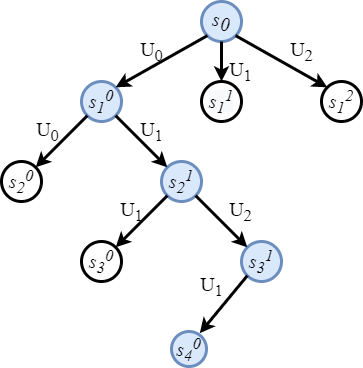
\includegraphics[width=0.5\textwidth]{Figures/tree_example.png}
  \caption{The tree representation (along the arc with blue-shaded circles) of the unitary described in Eqns. (\ref{eq:U1U3U1U2}) and (\ref{eq:U1U3U1U2_list}). We can also see that some of the possible branches along the blue-node path are pruned, leading to the size of operation pool at some node smaller than the total number of possible choices c = $\vert \mathcal{C}\vert$}
  \label{fig:treeexample}
\end{figure}

The performance of the quantum circuit can be evaluated from the loss or reward, where the reward is just the negative of the loss. Both are functions of $P$, and the parameters of the chosen operations $\boldsymbol{\theta}$:
\begin{equation}
    \mathcal{L}(\mathcal{P},\boldsymbol{\theta})=L(\mathcal{P}, \boldsymbol{\theta})+\lambda
\end{equation}

\begin{equation}
    \mathcal{R}(\mathcal{P},\boldsymbol{\theta})=R(\mathcal{P}, \boldsymbol{\theta})-\lambda,
\end{equation}
where $\lambda$ is some penalty function that may only appear when certain circuit structures appear, as well as other kinds of penalty terms, like penalty on the sum of absolute value of weights or the number of certain type of gates in the circuit. The purpose of the penalty term $\lambda$ is to `sway' the search algorithm from structures we do not desire.
%\textcolor{red}{can you motivate this $\lambda$ penalty term a bit better?}. 
Instead of storing all the operation parameters for each different quantum circuit, we share the parameters for a single operation at a certain location. That is, we have a multidimensional array of shape $(p, c, l)$, where $l$ is the maximum number of parameters for the operations in the operation pool. In Eqn~\ref{eq:U1U3U1U2} and Fig~\ref{fig:treeexample}, if the $U_i$ gate can be considered as the $U3$ gate \cite{nielsen00}:
\begin{equation}
U 3(\theta, \phi, \lambda)=\left[\begin{array}{cc}
\cos \left(\frac{\theta}{2}\right) & -e^{i \lambda} \sin \left(\frac{\theta}{2}\right) \\
e^{i \phi} \sin \left(\frac{\theta}{2}\right) & e^{i(\phi+\lambda)} \cos \left(\frac{\theta}{2}\right)
\end{array}\right]
\end{equation}
then in this case $l=3$

To reduce the space required to store the parameters of all possible quantum circuits, for a quantum circuit with operation $k$ at layer $i$, the parameter is the same at that layer for that specific operation is the same for all other circuits with the same operation at the same location, which means we are sharing the parameters of the unitaries in the operation pool with other circuits. For example, in Fig.\ref{fig:treeexample}, besides the blue-node arc $\mathcal{P}=[U_0, U_1, U_2, U_1]$, there are also other paths, like $\mathcal{P}^{'} = [U_0, U_1, U_1, \cdots]$, and since the first two operations in $\mathcal{P}$ and $\mathcal{P}^{'}$ are the same, then we will share the parameters of $U_0$ and $U_1$ between these two circuits by setting the parameters to be the same for the two $U_0$s and $U_1$s in both circuits, respectively.
%\textcolor{red}{I'm not sure what you're trying to say here... Or whether it is important. This needs to be clarified} 
Such a strategy is often called ``parameter-sharing'' or ``weight-sharing'' in the neural architecture search literature.

As shown in Fig~\ref{fig:treeexample} and mentioned earlier, the process of composing or searching a circuit can be formulated in the form of the tree structure. For example, if we start from an empty list $P = [\;]$ with maximal length four and an operation pool with three elements $C = \{U_0, U_1, U_2\}$, 
%\textcolor{red}{why did you choose 4 and 3? Is this arbitrary, or was this what was used for this work throughout the paper? Or is is a way of easing the reader into the technique and notation?}.
then the state of the root node of our search tree will be the empty list $s_0^0 = [\;]$. The root node will have three possible actions (if there are no restrictions on what kind of operations can be chosen), which will lead us to three children nodes with states $s_1^0 = [U_0]=[0], s_1^1 = [U_1]=[1], s_1^2=[U_2] = [2]$. For each of these nodes, there will be a certain number of different operations that can be chosen to append the end of the list, depending on the specific restrictions. There will always be a ``placeholder'' operation that can be chosen if all other operations fail to meet the restrictions. The penalty resulting from the number of ``placeholder'' operations will only be reflected in the loss (or reward) of the circuit. The nodes can always be expanded with different actions, leading to different children, until the maximum length of the quantum circuit has been reached, which will give us the leaf node of the search tree. 
%\textcolor{red}{Can we put a really simply tree figure here, with maybe three levels to help explain this? Maybe just one of the trees from Fig. (1)?}

The process of choosing operations at each layer can be viewed as a both a \textit{local} and \textit{global} multi-armed bandit (MAB):
\begin{itemize}
    \item \textit{Local MAB}: The choice of unitary operations at each layer can be considered a \textit{local} MAB. That is, different unitary operations can be treated as different ``arms'' of the bandit;
    \item \textit{Global MAB}: We can also treat the composition of the entire quantum circuit as a \textit{global} MAB. That is, different quantum circuits can be viewed as different ``arms'' of the global bandit.
\end{itemize}


%The choice of a whole quantum circuit can also be viewed as a multi-armed bandit with the arms being different quantum circuits, which is called the \textit{global} MAB. Such a formulation enables the application of the na\"ive sampling strategy with the na\"ive assumption \cite{CMAB_RTS} when exploring different combinations of operations in a quantum circuit. 
%\textcolor{red}{This wasn't very clear to me. I think the explanation for both the local and global MAB need to be expanded a bit.}

\subsection{Monte Carlo tree search (MCTS), nested MCTS and the na\"ive assumption}
Monte Carlo tree search (MCTS) is a heuristic search algorithm for a sequence decision process. It has achieved great success in other areas, including defeating the 18-time world champion Lee Sedol in the game of Go \cite{AlphaGoDBLP:journals/nature/SilverHMGSDSAPL16, AlphaGoZeroDBLP:journals/nature/SilverSSAHGHBLB17}. Generally, there are four stages in a single iteration of MCTS (see Fig.~\ref{fig:mcts}) \cite{MCTS_for_game10.5555/3022539.3022579}:
\begin{figure}[]
  \centering
  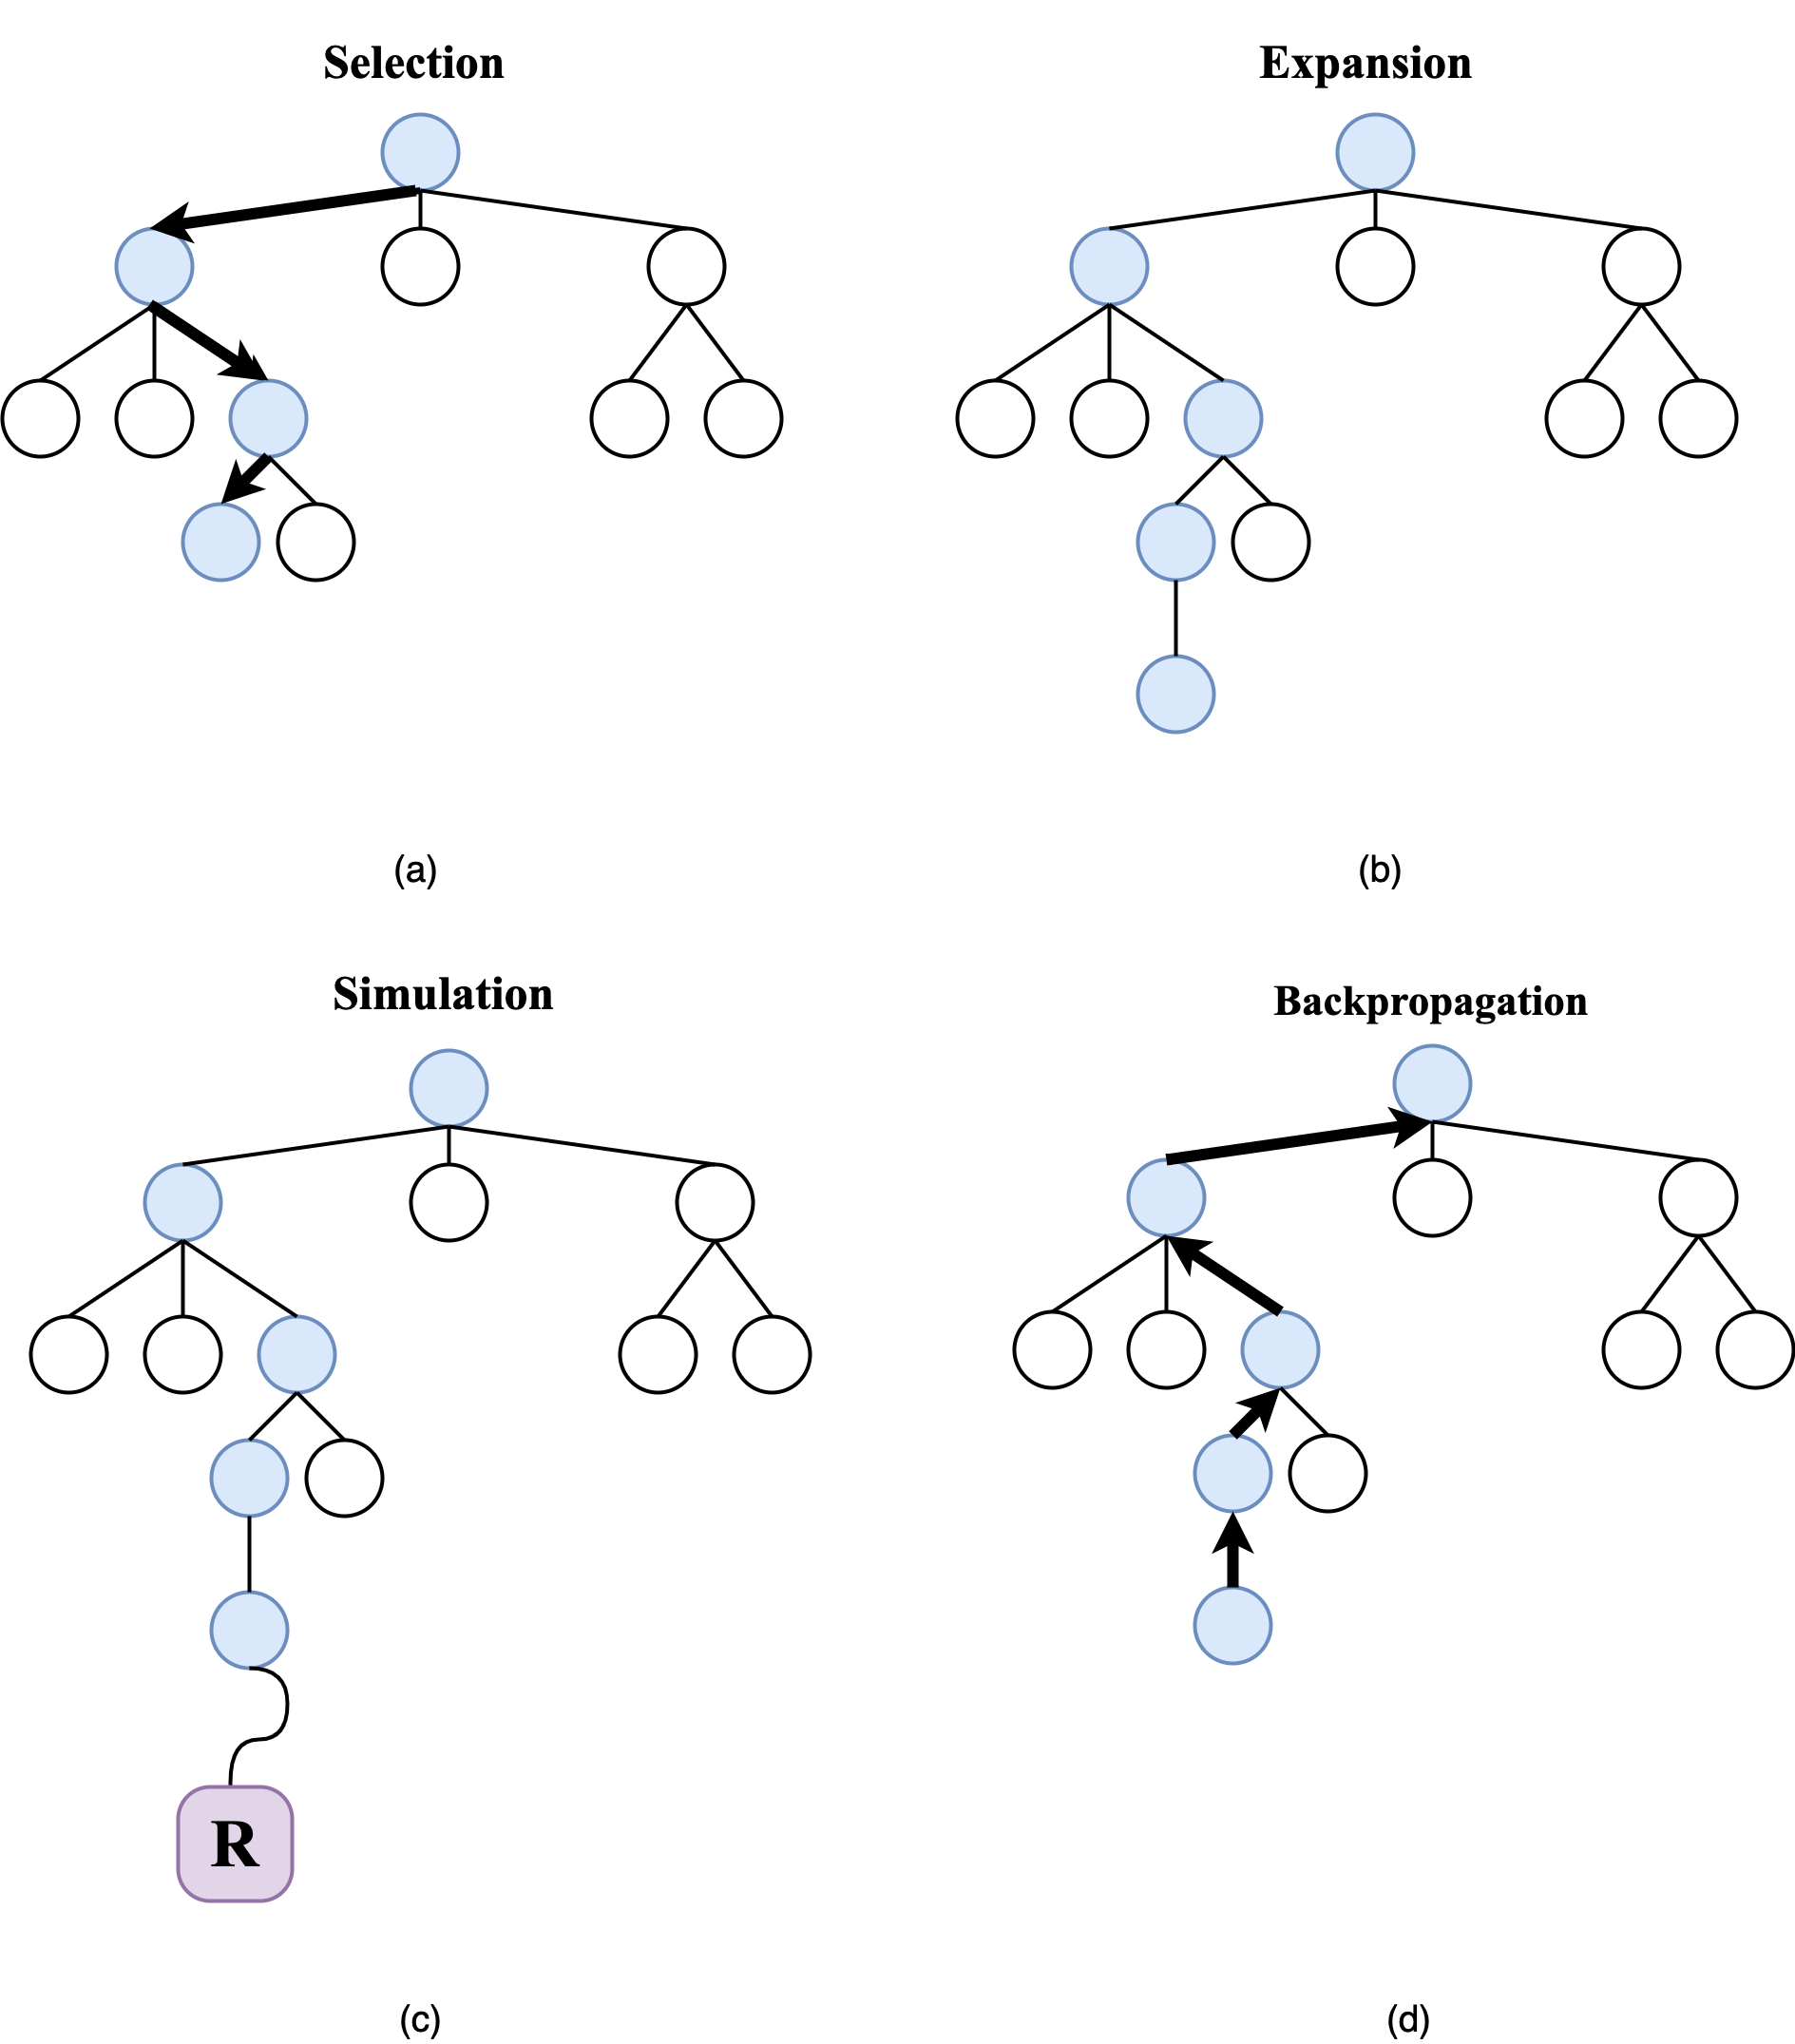
\includegraphics[width=0.8\textwidth]{Figures/mcts.png}
  \caption{Four stages of Monte Carlo tree search. From left to right, up to down: Selection: Go down from the root node to a non fully expanded leaf node; Expansion: Expand the selected node by taking an action; Simulation: Simulate the game, which in our case is the quantum circuit, to obtain reward information \textbf{R}; Backpropagation: Back-propagate the reward information along the path (arc) taken.}
  \label{fig:mcts}
\end{figure}

\begin{itemize}
    \item \textsc{Selection:}(Fig.\ref{fig:mcts}(a)) In the selection stage, the algorithm will, starting from the root of the tree, find a node at the end of an arc (a path from the root of the tree to the leaf node, the path marked by bold arrows and blue circles in Fig \ref{fig:mcts}). The nodes along the arc are selected according to some policy, often referred as the ``selection policy'', until a non fully expanded node or a leaf node is reached. If the node is a leaf node, i.e after selecting the operation for the last layer of the quantum circuit, we can directly jump to the simulation stage to get the reward of the corresponding arc. If the node is not a leaf node, i.e the node is not fully expanded, then we can progress to the next stage;
    \item \textsc{Expansion:}(Fig.\ref{fig:mcts}(b)) In the expansion stage, at the node selected in the previous stage, we choose a previously unvisited child by choosing a previously unperformed action. We can see from the upper right tree in Fig \ref{fig:mcts} that a new node has been expanded at the end of the arc; %\textcolor{red}{I don't understand how to corresponds to the second part of Fig. (1)?}
    \item \textsc{Simulation:}(Fig.\ref{fig:mcts}(c)) In the simulation stage, if the node obtained from the previous stages is not a leaf node, we continue down the tree until we have reached a leaf node, i.e finish choosing the operation for the last layer. After we have the leaf node, we simulate the circuit and obtain the loss $\mathcal{L}$ (or reward $\mathcal{R}$). Usually, the loss $\mathcal{L}$ is required to update the parameters in the circuit;
    \item \textsc{Backpropagation:}(Fig.\ref{fig:mcts}(d)) In this stage, the reward information obtained from the simulation stage is back-propagated through the arc leading from the root of the tree to the leaf node, and the number of visits as well as the (average) reward for each node along the arc is be updated.
\end{itemize}

The nested MCTS algorithm \cite{nestedmontecarlosearch} is based on the vanilla MCTS algorithm. However, before selecting the best child according to the selection policy, a nested MCTS will be performed on the sub-trees with each child as the root node. Then the best child will be selected according to the selection policy with updated reward information, see Fig.~\ref{fig:nestedmcts}.

\begin{figure}[H]
  \centering
  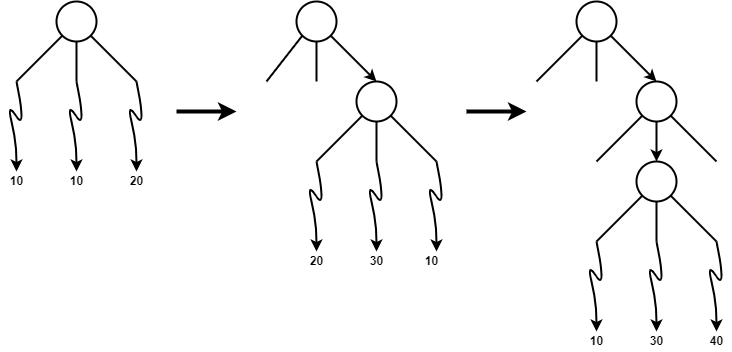
\includegraphics[width=0.8\textwidth]{Figures/nmcs.png}
  \caption{Nested Monte Carlo tree search. Left: The root node has three possible actions, which in this case are unselected initially. We perform MCTS on all three children nodes (generated by the three possible actions) to update their reward information. In this case, the right child has the highest reward. Middle: After selecting the right side child node, we perform the same MCTS on all three possible children nodes as before, which gives updated reward information. In this case the middle child node has the highest reward, meaning that at this level we expand the middle child node. Right: Similar operations as before. If we only perform nested MCTS at the root node level, then it will be a level-1 nested MCTS.}
  \label{fig:nestedmcts}
\end{figure}



We denote a quantum circuit with $p$ layers $\mathcal{P} = [k_1,\cdots, k_p]$, with each layer $k_i$ having a search space no greater than $\vert \mathcal{C} \vert = c$ (where $c$ is the number of possible unitary operations, as defined earlier). Then each choice for layer $k_i$ is a \textit{local arm} for the \textit{local MAB}, $MAB_i$. The set of these choices is also denoted as $k_i$. The combination of all $p$ layers in $\mathcal{P}$ forms a valid quantum circuit, which is called a \textit{global arm} of the \textit{global MAB, $MAB_g$}. 

Since the global arm can be formed from the combination of the local arms, if we use the na\"ive assumption \cite{CMAB_RTS}, the global reward $r_g$ for $MAB_g$ can be approximated by the sum of the reward of local MABs, and each local reward only depends on the choice made in each local MAB. This also means that, if the global reward is more easily accessed than the local rewards, then the local rewards can be approximated from the global reward. With the na\"ive assumption, we can have a linear relationship between the global reward and local rewards:
\begin{equation}
    R_{global} = \frac{1}{p}\sum_{i=1}^p R_i
\end{equation}
Since when searching for quantum circuits, we have no access to the reward distribution of individual unitary operations. However, we can apply the na\"ive assumption to approximate those rewards (``local reward'') with the global reward: 
\begin{equation}
    R_{i} \approx R_{global}
\end{equation}
where $R_{i}$ is the reward for pulling an arm at \textit{local $MAB_i$} and $R_{global}$ is the reward for the global arm.
%\textcolor{red}{but how, by just a simple division of the global reward, or is there some weighting that needs to be taken into account?} 
Also, if we use the na\"ive assumption, we will not need to directly optimise on the large space of global arms as in  traditional MABs. Instead, we can apply MCTS on the local MABs to find the best combination of local arms.

In the original work on nested MCTS~\cite{nestedmontecarlosearch}, a random policy was adopted for sampling. In this paper we will instead change it to the famous UCB policy~\cite{UCB_paper_10.5555/944919.944941}. Given a local $MAB_i$, with the set of all the possible choices $k_i$, the UCB policy can be defined as:
\begin{equation}
    UCB: \argmax_{arm_j\in k_i} \Bar{r}(k_i, arm_j) + \alpha \sqrt{\frac{2\ln n_i}{n_j}}
\end{equation}
where $\Bar{r}(k_i, arm_j)$ is the average reward for $arm_j$ (i.e the reward for operation choice $U_j$  for layer $k_i$) in local $MAB_i$, $n_i$ is the number of times that $MAB_i$ has been used and $n_j$ is the number of times that $arm_j$ has been pulled. The parameter $\alpha$ provides a balance between exploration ($\sqrt{\frac{2\ln n_i}{n_j}}$) and exploitation ($\Bar{r}(k_i, arm_j$)). The UCB policy modifies the reward which the selection of action will be based on. 



For small $\alpha$, the actual reward from the bandit will play a more important role in the UCB modified rewards, which will lead to selecting actions with previously observed high rewards. When $\alpha$ is large enough, the second term, which will be relatively large if $MAB_i$ has been visited many times but $arm_j$ of $MAB_i$ has only been pulled a small number of times, will have more impact on the modified reward, leading to a selection favoring previously less visited actions.
%\textcolor{red}{I'm finding it hard to get an intuition from Eq. (7). I know we discussed it in our meetings, but I think we need to include a bit more description behind Eq. (7).}
%With naïve assumption \cite{CMAB_RTS}, we treat the selection of operations at each layer of the circuit as a local multi-armed bandit, and the selection of different circuit structure as a global multi-armed bandit, and the reward for global MAB is a linear function of the local MABs. Since we can calculate the reward of a circuit (global MAB) with the pre-defined loss/reward function, then we can just assign the reward of the global MAB to the selected actions of each local MAB, then take the average with respect to the number of times the corresponding action has been taken. Then we can prune the children nodes if the average reward of the children node is smaller than a certain percentage of the reward of the parent node.

\subsection{QAS with Nested Na\"ive MCTS}
%\textcolor{red}{I struggled to get much out of this section. Have you seen many QML papers that have a section that is just algorithm pseudo code? I think we need to expand this a bit and explain how things fit together. }

%Searching quantum ansatzes with MCTS requires Algorithms 1$\sim$4 \textcolor{red}{Why? Did you mean: Searching quantum ansatzes with MCTS can be accomplished by defining Algorithms 1$\sim$4?}. In a single iteration, the search algorithm will:
%\begin{enumerate}
%    \item Sample a batch of quantum circuits with the $SampleArc$ algorithm;
%    \item Calculate the gradients of the circuits in the sampled batch;
%    \item Calculate the average gradient of the batch gradients;
%    \item Update the shared parameters according to the average gradient;
%    \item Find the best arc with the $ExploitArc$ algorithm and updated parameters;
%\end{enumerate}

%When there are parameters in the candidate operations, we could perform several warm-up iterations before actually searching. The steps for the warm-up iterations are the same as those for the searching iterations, except in the first step where the $SampleArc$ algorithm will be replaced by random sampling. \textcolor{red}{why is this?}
    
Generally, a single iteration for the search algorithm will include two steps for non-parameterized circuits, and two more parameter-related steps for parameterized quantum circuits. The set of parameters, which will be referred to as the parameters of the super circuit, or just parameters, in the following algorithms, follow the same parameter sharing strategy as described in Section 2.1. That is, if the same unitary operation (say, $U_2$) appears in the same location (say, layer \#5) across different quantum circuits, then the parameters are the same, even for different circuits. Also, with parameterized quantum circuits (PQC), it is common practice to ``warm-up'' the parameters by randomly sampling a batch of quantum circuits, calculating the averaged gradient, and update the parameters according to the averaged gradient, to get a better start for the parameters during the search process. During one iteration of the search algorithm, we have:
\begin{enumerate}
    \item Sample a batch of quantum circuits from the super circuit with Algorithm \ref{alg:sampleArc};
    \item (For PQCs) Calculate the averaged gradients of the sampled batch, add noise to the gradient to guide the optimizer to a more ``flat'' minimum if needed;
    \item (For PQCs) Update the super circuit parameters according to the averaged gradients;
    \item Find the best circuit with Algorithm \ref{alg:exploitArc}.
\end{enumerate}

We could also set up an early-stopping criteria for the search. That is, when the reward of the circuit obtained with Algorithm \ref{alg:exploitArc} meets a pre-set standard, we will stop the search algorithm and return the circuit that meet such standard (and further fine-tune the circuit parameters if there are any).

With the na\"ive assumption, which means the reward is evenly distributed on the local arms pulled for a global MAB, we can impose a prune ratio during the search. That is, given a node that has child nodes, if the average reward of a child node is smaller than a ratio, or percentage, of the average reward of the said node, then this child node will be removed from the set of all children, unless the number of children reached the minimum requirement.

\begin{algorithm}
\caption{SampleArc}\label{alg:sampleArc}
\begin{algorithmic}
\Require sample policy $Policy$, parameters of the super circuit $param$, number of rounds in sampling $N$
\Ensure list representation $\mathcal{P}$ of quantum circuit
\State $curr \gets GetRoot(Tr)$ \Comment{Starting from the root node of the tree $Tr$}
\State $i\gets0$ \Comment{Counter}
\While{$i<N$}
\State $ExecuteSingleRound(curr, Policy, param)$
\State $i\gets i+1$
\EndWhile
\While{$curr$ is not leaf node}
\State $curr\gets SelectNode(curr, Policy)$
\EndWhile
\State $\mathcal{P}\gets GetListRepresentation(curr)$
\end{algorithmic}
\end{algorithm}

\begin{algorithm}[H]
\caption{ExploitArc}\label{alg:exploitArc}
\begin{algorithmic}
\Require exploit policy $Policy$, parameters of the super circuit $param$, number of rounds in exploitation $N$
\Ensure list representation $\mathcal{P}$ of quantum circuit
\State $curr \gets GetRoot(Tr)$ \Comment{Starting from the root node of the tree $Tr$}
\While{$curr$ is not leaf node}
\State $i\gets0$ \Comment{Counter}
\While{$i<N$}
\State $ExecuteSingleRound(curr, Policy, param)$
\State $i\gets i+1$
\EndWhile
\State $curr\gets SelectNode(curr, Policy)$
\EndWhile
\State $\mathcal{P}\gets GetListRepresentation(curr)$
\end{algorithmic}
\end{algorithm}

\begin{algorithm}
\caption{SelectNode}\label{alg:selectChild}
\begin{algorithmic}
\Require current node $n$, selection policy $Policy$
\Ensure selected node $n'$

\If{$n$ is fully expanded}
    \State $PruneChild(n)$ \Comment{Prune children nodes according to certain threshold}
    \State $n' \gets GetBestChild(n, Policy)$  \Comment{Select the best child}
\Else
    \State $n' \gets ExpandChild(n)$ \Comment{Expand the node}
\EndIf
\end{algorithmic}
\end{algorithm}

\begin{algorithm}[H]
\caption{ExecuteSingleRound}\label{alg:executeSingleRound}
\begin{algorithmic}
\Require current node $n$, selection policy $Policy$, parameters of the super circuit $param$
\Ensure leaf node $n'$
\State $n'\gets n$
\While{$n'$ is not leaf node}
\State $n'\gets SelectNode(n', Policy)$
\EndWhile
\State $R \gets Simulation(n', param)$  \Comment{Obtain reward from simulation}
\State $Backpropagate(n', R)$ \Comment{Backpropagate the reward information along the arc}
\end{algorithmic}
\end{algorithm}




\section{Numerical Experiments and Results}\label{experiments}
\subsection{Searching for the encoding circuit of [[4,2,2]] quantum error detection code}\label{422}

%\textcolor{red}{You need to introduce the [[4,2,2]] code here. Why is it useful to consider, what can it do, why is it useful as a quantum test bed? Cite some of the important literature around the [[4,2,2]] code. }
The [[4,2,2]] quantum error detection code is a simple quantum error detection code, which needs 4 physical qubits for 2 logical qubits and has a code distance 2. It is the smallest stabilizer code that can detect X- and Z-errors \cite{qec_intro_guide}. One possible set of code words for the [[4,2,2]] error detection code is:


\begin{equation}
\mathcal{C}_{[[4,2,2]]}=\operatorname{span}\left\{\begin{array}{l}
|00\rangle_{L}=\frac{1}{\sqrt{2}}(|0000\rangle+|1111\rangle) \\
|01\rangle_{L}=\frac{1}{\sqrt{2}}(|0110\rangle+|1001\rangle, \\
|10\rangle_{L}=\frac{1}{\sqrt{2}}(|1010\rangle+|0101\rangle) \\
|11\rangle_{L}=\frac{1}{\sqrt{2}}(|1100\rangle+|0011\rangle)
\end{array}\right\}
\end{equation}

The corresponding encoding circuit is shown in Fig \ref{fig:lit422}.

\begin{figure}[H]
  \centering
  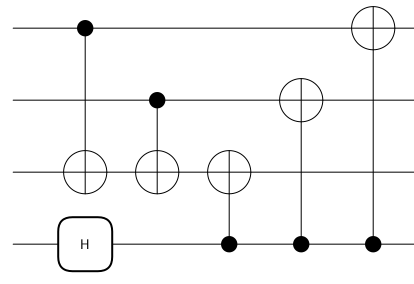
\includegraphics[width=0.5\textwidth]{Figures/422_from_literature.png}
  \caption{Encoding circuit of the [[4,2,2]] code \cite{qec_intro_guide} to detect X- and Z-errors. It needs 4 physical qubits for 2 logical qubits and has a code distance 2}
  \label{fig:lit422}
\end{figure}

Quantum error detection and correction is vital to large-scale fault-tolerant quantum computing. By searching for the encoding circuit of the [[4,2,2]] error detection code, we demonstrate that our algorithm has the potential to automatically find  device-specific encoding circuits of quantum error detection and correction codes for future quantum processors.

\subsubsection{Experiment Settings}
When searching for the encoding circuit of the [[4,2,2]] quantum error correction code, we adopted an operation pool consisting of only non-parametric operations: the Hadamard gate on each of the four qubits and CNOT gates between any two qubits. The total size of the operation pool is $4 + \frac{4!}{2!\times2!}\times2=16$. When there are 6 layers in total, the overall size of the search space is $16^6\approx1.67\times10^7$.

The loss function for this task is based on the fidelity between the output state of the searched circuit and the output generated by the encoding circuit from Section 4.3 of \cite{qec_intro_guide} (also shown in Fig.~\ref{fig:lit422}) when input states taken from the set of Pauli operator eigenstates and the magic state $\mathcal{S}$ are used:
\begin{equation}
    \mathcal{S}=\{\vert 0 \rangle, \vert 1 \rangle, \vert + \rangle, \vert - \rangle, \vert +i \rangle, \vert -i \rangle, \vert T \rangle\}
\end{equation}
where $\vert T \rangle = \frac{\vert 0 \rangle + e^{i\pi/4}\vert 1 \rangle}{\sqrt{2}}$.



%\textcolor{red}{Do we need the code words to be defined?} The code words for the [[4,2,2]] code are given by~\cite{qec_intro_guide}:


The input states (initialised on all four qubits) are
\begin{equation}
    \mathcal{I}_{[[4,2,2]]} = \{\vert \varphi_1 \rangle \otimes \vert \varphi_2 \rangle\otimes\vert 00\rangle \; \vert \; \vert \varphi_1 \rangle, \vert \varphi_2 \rangle \in \mathcal{S}\}
\end{equation}

We denote the unitary on all four qubits shown in Fig.~\ref{fig:lit422} as $U_{[[4,2,2]]}$, and the unitary from the searched circuit as $U_{Searched\;[[4,2,2]]}$, which is a function of the structure $\mathcal{P}_{Searched\;[[4,2,2]]}$. The loss and reward function can then be expressed as:
\begin{equation}
    L_{[[4,2,2]]} = 1-\frac{1}{\vert \mathcal{I}_{[[4,2,2]]} \vert}\sum_{\vert \psi_i\rangle\in  \mathcal{I}_{[[4,2,2]]}} \langle \psi_i \vert U_{Searched\;[[4,2,2]]}^{\dagger} O_{[[4,2,2]]}(\vert \psi_i\rangle)  U_{Searched\;[[4,2,2]]} \vert \psi_i\rangle
\end{equation}
\begin{equation}
    R_{[[4,2,2]]} = 1-L_{[[4,2,2]]}
\end{equation}
where
\begin{equation}
    O_{[[4,2,2]]}(\vert \psi_i\rangle) = U_{[[4,2,2]]} \vert \psi_i\rangle \langle \psi_i \vert U_{[[4,2,2]]}^{\dagger},\; \vert \psi_i\rangle\in  \mathcal{I}_{[[4,2,2]]}
\end{equation}



The circuit simulator used in this and the following numerical experiments is Pennylane \cite{bergholm2020pennylane}.
\subsubsection{Results}
To verify whether the search algorithm will always reach the same solution, we ran the search algorithm twice, and both times the algorithm found an encoding circuit within a small numbers of iterations (Fig.~\ref{fig:422_reward}), although the actual circuit are different from each other, as shown in Fig.~\ref{fig:422_circ}. The search process that gave the circuit in Fig \ref{fig:422_first_circ} met the early-stopping criteria in only four iterations, and the search process that gave the circuit in Fig \ref{fig:422_second_circ} met the early-stopping criteria in only eight iterations, as shown in Fig.~\ref{fig:422_reward}.
%\textcolor{red}{My first impression here is that we should explain why the search algorithm was only run twice, and what went into choosing this. Also, trying to explain why the reward graph too a different number of epochs for the two different search cases. }
\begin{figure}[H]
    \centering
    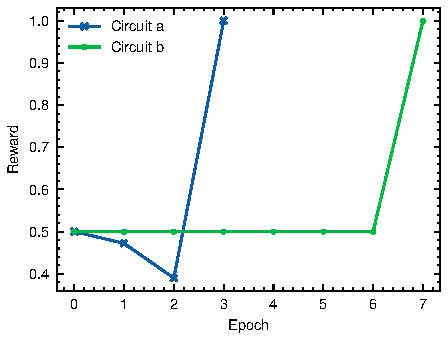
\includegraphics[width=0.8\textwidth]{Figures/fig_422_rewards_1_2.pdf}
    \caption{Rewards when searching for encoding circuits of the [[4,2,2]] code. We can see that in both cases the algorithm was able find the encoding circuit that generated the required code words in just a few iterations. `Circuit a' refers to the search rewards for the circuit in Fig \ref{fig:422_first_circ} and `Circuit b' refers to the search rewards for the circuit in Fig \ref{fig:422_second_circ}.}\label{fig:422_reward}
\end{figure}
%Since there are random elements involved during the search process, the circuits produced during the two runs of the algorithm are different, as seen in Fig.~\ref{fig:422_circ}. However, these two circuits both reach the required code space.
\begin{figure}[H]
    \centering
    \begin{subfigure}[b]{0.48\textwidth}
        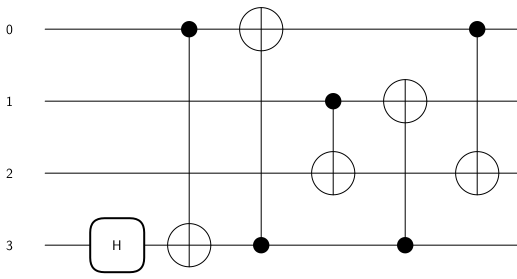
\includegraphics[width=\textwidth]{Figures/422_searched_1.png}
        \caption{}
        \label{fig:422_first_circ}
    \end{subfigure}
    ~ %add desired spacing between images, e. g. ~, \quad, \qquad, \hfill etc. 
      %(or a blank line to force the subfigure onto a new line)
    \begin{subfigure}[b]{0.48\textwidth}
        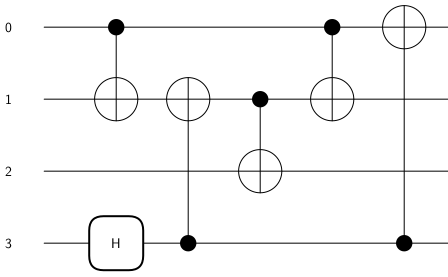
\includegraphics[width=0.9\textwidth]{Figures/422_searched_2.png}
        \caption{}
        \label{fig:422_second_circ}
    \end{subfigure}
    \caption{Two different encoding circuits of the [[4,2,2]] code produced by the search algorithm.}\label{fig:422_circ}
\end{figure}

\subsection{Solving linear equations}
The variational quantum linear solver (VQLS), first proposed in \cite{Bravo-Prieto_undated-oq}, is designed to solve linear systems $Ax=b$ on near term quantum devices. Instead of using quantum phase estimation like the HHL algorithm \cite{HHL}, which is unfeasible on near term devices due to large circuit depth, VQLS adopts a variational circuit to prepare a state $\ket{x}$ such that 
\begin{equation}
    A\ket{x} \propto \ket{b}
\end{equation}
In this section, we will task our algorithm to automatically search for a variantional circuit to prepare a state $\ket{x}$ to solve $Ax = b$ with A in the form of 
\begin{equation}
    A = \sum_l c_l A_l
\end{equation}
where $A_l$ are unitaries, and $\ket{b} = H^{\otimes n}\ket{\mathbf{0}}$.

We will also adopt the local cost function $C_L$ described in \cite{Bravo-Prieto_undated-oq}:
\begin{equation}\label{eqn:vqls_local_loss}
C_{L}=1-\frac{\sum_{l, l^{\prime}} c_{l} c_{l^{\prime}}^{*}\bra{0}V^{\dagger} A_{l^{\prime}}^{\dagger} U P U^{\dagger} A_{l} V\ket{0}}{\sum_{l, l^{\prime}} c_{l} c_{l^{\prime}}^{*}\bra{0}V^{\dagger} A_{l^{\prime}}^{\dagger} A_{l} V\ket{0}}
\end{equation}
where $U=H^{\otimes n}$, $V$ is the (searched) variational circuit that can produce the solution state $V\ket{0} = \ket{x}$, and $P=\frac{1}{2}+\frac{1}{2 n} \sum_{j=0}^{n-1} Z_{j}$ \cite{pennylane_vqls}.

\subsubsection{Experiment Settings}
The linear system to be solved in our demonstration is:
\begin{equation}
    A = \zeta  I + J X_1 + J X_2  + \eta Z_3 Z_4
\end{equation}
\begin{equation}
    \ket{b} = H^{\otimes 4}\ket{0}
\end{equation}
with $J = 0.1, \zeta = 1, \eta = 0.2$.
The loss function we adopted follows the local loss $C_L$ in Eqn.~\ref{eqn:vqls_local_loss}. However, since the starting point of the loss values often has a magnitude of $10^{-2}\sim 10^{-3}$, we will need scaling in the reward function:
\begin{equation}
    \mathcal{R} = e^{-10 C_L}-\lambda
\end{equation}
where $\lambda$ is a penalty term depending on the number of Placeholder gates in the circuit. The operation pool consists of CNOT gates between neighbouring two qubits as well as the first and fourth qubits, the Placeholder and the single qubit rotation gate Rot \cite{nielsen00}:
\begin{equation}
Rot(\phi, \theta, \omega)=R_Z(\omega) R_Y(\theta) R_Z(\phi)=\left[\begin{array}{cc}
e^{-i(\phi+\omega) / 2} \cos (\theta / 2) & -e^{i(\phi-\omega) / 2} \sin (\theta / 2) \\
e^{-i(\phi-\omega) / 2} \sin (\theta / 2) & e^{i(\phi+\omega) / 2} \cos (\theta / 2)
\end{array}\right]
\end{equation}
The size of the operation pool $c = \vert \mathcal{C}\vert = 16$, and number of layers $p = 10$, giving us a search space of size $\vert \mathcal{S} \vert = 10^{16}$. There is also an additional restriction of maximum number of CNOT gates in the circuit, which is 8, the number of CNOT gates required to created two layers of circular entanglement.
\subsubsection{Results}

\begin{figure}[H]
    \centering
    \begin{subfigure}[t]{0.48\textwidth}
        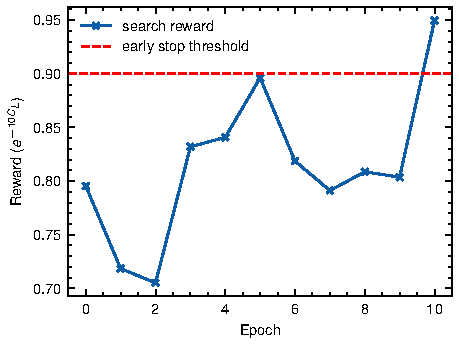
\includegraphics[width=\textwidth]{Figures/fig_vqls_4q_search_rewards.pdf}
        \caption{Search rewards for VQLS. The change of rewards with respect to the iterations is shown. We can see that the reward quickly reached the early stopping threshold at iteration 10. In the VQLS case, the reward is scaled since the initial reward with random sampled circuit structure and parameters is already at the magnitude of $10^{-2}$.}
        \label{fig:vqls_4q_search}
    \end{subfigure}
    ~ %add desired spacing between images, e. g. ~, \quad, \qquad, \hfill etc. 
      %(or a blank line to force the subfigure onto a new line)
    \begin{subfigure}[t]{0.48\textwidth}
        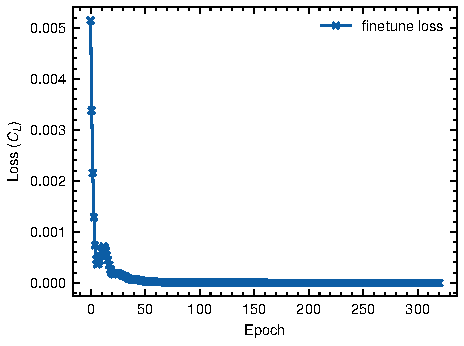
\includegraphics[width=\textwidth]{Figures/fig_vqls_4q_finetune.pdf}
        \caption{Fine-tune loss for the VQLS circuit.After the searched stopped at iteration 10 as shown in Fig~\ref{fig:vqls_4q_search}, the structure of the circuit is left unchanged and its parameters are optimized to achieve smaller losses. The final loss of the optimized parameters is very close to 0.}
        \label{fig:vqls_4q_finetune}
    \end{subfigure}
    \caption{The search rewards and fine-tune loss for VQLS experiment. }\label{fig:vqls_search_finetune}
\end{figure}

\begin{figure}[H]
  \centering
  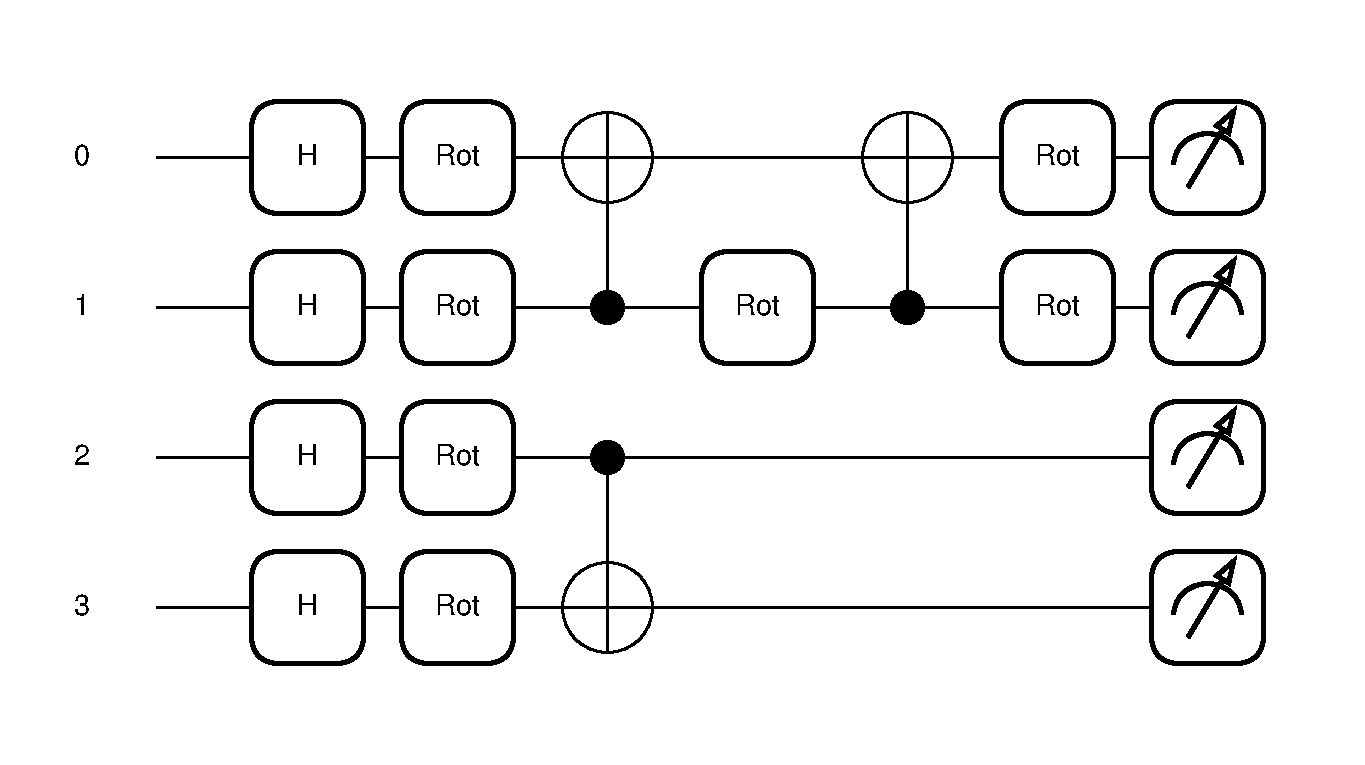
\includegraphics[width=0.75\textwidth]{Figures/fig_vqls_circ.pdf}
  \caption{Circuit searched for the VQLS problem.}
  \label{fig:vqls_circ}
\end{figure}

\begin{figure}[H]
  \centering
  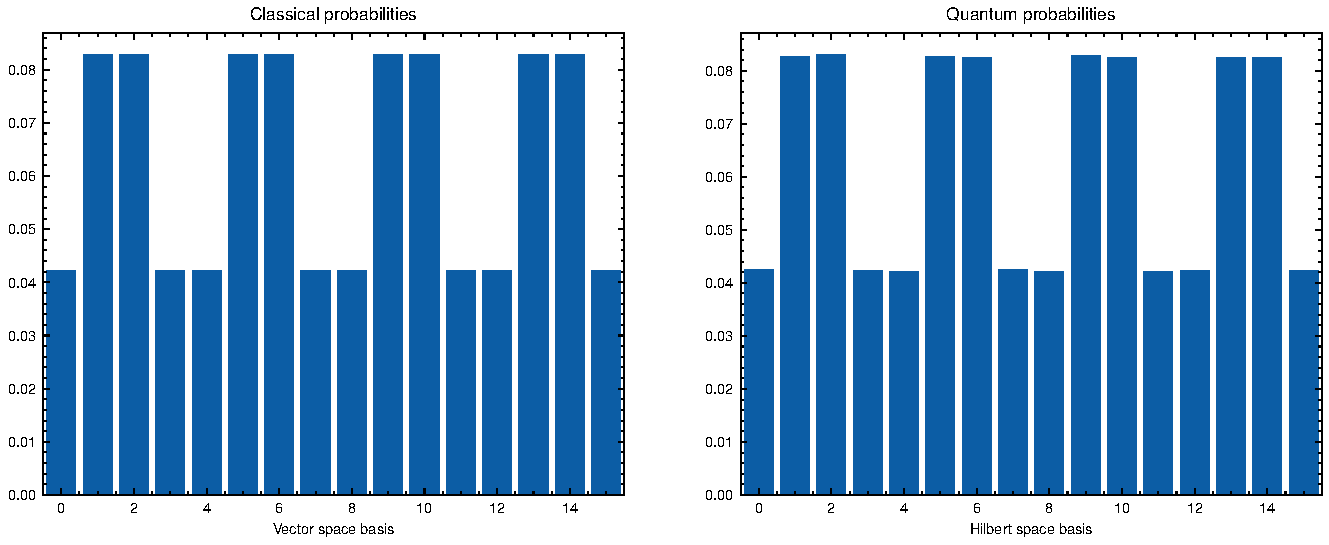
\includegraphics[width=0.95\textwidth]{Figures/fig_vqls_search_results_compare.pdf}
  \caption{Comparison between classical probabilities of the normalized solution vector $\frac{x}{||x||}$ for $Ax = b$ (left), and the probabilities obtained by sampling the state $\ket{x}$ produced by the trained circuit in Fig~\ref{fig:vqls_circ} (right). The number of shots for measurement is $10^6$. We can see that the quantum results is very close to the classically obtained ones, proving that our algorithm can be indeed applied to finding variational ans\"atz for VQLS problems.}
  \label{fig:vqls_results_compare}
\end{figure}

The search rewards as well as fine-tune losses are shown in Fig~\ref{fig:vqls_search_finetune}. We can see that the search algorithm can produce a circuit with high reward (exceeds the threshold) quickly and the loss of the optimized parameters can reach close to 0. Although facing a large search space, our algorithm can still find a circuit (shown in Fig~\ref{fig:vqls_circ}) that minimizes the loss function (Fig~\ref{fig:vqls_4q_finetune}) and leads us to results close to the classical solution. A comparison of the results obtained by directly solving the linear equation $Ax=b$ and the results obtained by sampling the state $\ket{x}$ produced by the searched circuit is shown in Fig~\ref{fig:vqls_results_compare}. 


\subsection{Search for quantum chemistry ansatzes}\label{h2}


%\textcolor{red}{[Need a better lead in sentence for quantum chemistry here: Recent progress on solving the ground state energy problem on a quantum computer has been made with near-term parameterised circuits~\cite{}...]}
Recently, there has been a lot of progress made on finding the ground state energy of a molecule on a quantum computer with variational circuit, both on theoretical \cite{li2017efficient,mcclean2016theory,wecker2015progress} and experimental \cite{peruzzo2014variational,o2016scalable, colless2017implementing, kandala2017hardware, colless2018computation, dumitrescu2018cloud} front. 
Normally, when designing the ansatz for the ground energy problem either a physically plausible or a hardware efficient ansatz needs to be found. However, our algorithm provides an approach which can minimise the effort needed to carefully choose an ansatz and automatically design the circuit according to the device gate set and topology.

Generally speaking, solving the ground energy problem with quantum computers is an application of the variational principle \cite{sakurai_napolitano_2017}:
\begin{equation}
E_0 \leq \frac{\langle\tilde{0}|H| \tilde{0}\rangle}{\langle\tilde{0} \mid \tilde{0}\rangle} \label{eq:variational}
\end{equation}
where $H$ is the system Hamiltonian, $| \tilde{0}\rangle$ is the ``trail ket'' \cite{sakurai_napolitano_2017}, or ansatz, trying to mimic the real wave function at ground state with energy $E_0$, which is the smallest eigenvalue of the system Hamiltonian H. Starting from $\ket{0^{\otimes n}}$ for an $n-$qubit system, the ``trial ket'' can be written as a function of a set of (real) parameters $\theta$:
\begin{equation}
    \ket{\tilde{0}} = \ket{\varphi (\theta)} = U(\theta)\ket{0^{\otimes n}}
\end{equation}
Given an ansatz, the goal of optimization is to find a set of parameters $\theta$ that minimizes the right hand side of Eqn \ref{eq:variational}. However, in our research, the form of the trail wave function will no longer be fixed. We will not only vary the parameters, but also the circuit structure that represent the ansatz.

\subsubsection{Experiment settings}

\paragraph{Search an ansatz for finding the ground energy of $H_2$:}
In this experiment, we adopted the 4-qubit Hamiltonian $H_{hydrogen}$ for the hydrogen molecule $H_2$ generated by the Pennylane-QChem \cite{bergholm2020pennylane} package, when the coordinates of the two hydrogen atoms are $(0, 0, -0.66140414)$ and $(0, 0, 0.66140414)$, respectively, in atom units. The goal of this experiment is to find an ansatz that can produce similar states as the four-qubit Givens rotation for single and double excitation.
The unitary operator \footnote{see \url{https://pennylane.readthedocs.io/en/latest/code/api/pennylane.SingleExcitation.html}} that performs single excitation on a subspace spanned by $\{\ket{01}, \ket{10} \}$ can be written as 
\begin{equation}
U(\phi)=\left[\begin{array}{cccc}
1 & 0 & 0 & 0 \\
0 & \cos (\phi / 2) & -\sin (\phi / 2) & 0 \\
0 & \sin (\phi / 2) & \cos (\phi / 2) & 0 \\
0 & 0 & 0 & 1
\end{array}\right]
\end{equation}
And the transformation of the double excitation on the subspace spanned by $\{|1100\rangle,|0011\rangle\}$ is\footnote{see \url{https://pennylane.readthedocs.io/en/latest/code/api/pennylane.DoubleExcitation.html}} :
\begin{equation}
\begin{aligned}
&|0011\rangle \rightarrow \cos (\phi / 2)|0011\rangle+\sin (\phi / 2)|1100\rangle \\
&|1100\rangle \rightarrow \cos (\phi / 2)|1100\rangle-\sin (\phi / 2)|0011\rangle
\end{aligned}
\end{equation}

Following \cite{pennylane_dev_team_2021}, we initialised the circuit with the 4-qubit vacuum state $\vert \psi_0\rangle=\vert 0000\rangle$. We denote the unitary for the searched ansatz $U_{SearchedAnsatz}$, which is a function of its structure $\mathcal{P}_{SearchedAnsatz}$ and corresponding parameters. Then the loss and reward functions can be written as:
\begin{equation}
    L_{H_2} =\langle \psi_0 \vert U_{SearchedAnsatz}^{\dagger} H_{hydrogen} U_{SearchedAnsatz} \vert \psi_0\rangle
\end{equation}
\begin{equation}
    R_{H_2} = -L_{H_2}
\end{equation}

The operation pool consists of Placeholder gates, Rot gates and CNOT gates with a linear entanglement topology (nearest neighbour interactions). The maximum number of layers is 30, with maximum number of CNOT gates $30/2 = 15$, and no penalty term for the number of Placeholder gates:
\begin{equation}
    \mathcal{R}_{H_2, Pool\;1} = R_{H_2}
\end{equation}

Such settings of operation pool and number of layers will give us an overall search space of size $14^{30}\approx 2.42\times 10^{34}$. However, the imposed hard limits and gate limits will drastically reduce the size of the search space.


\paragraph{Search an ansatz for finding the ground energy of $LiH$}
The loss and reward functions for the $LiH$ task are similar to the $H_2$ one:
\begin{equation}
    L_{LiH} =\langle \psi_0 \vert U_{SearchedAnsatz}^{\dagger} H_{LiH} U_{SearchedAnsatz} \vert \psi_0\rangle
\end{equation}
\begin{equation}
    R_{LiH} = -L_{LiH}
\end{equation}
and the initial state is also the vacuum state $\ket{\psi_0} = \ket{0}^{\otimes 10}$. The Hamiltonian is obtained at bond length 2.969280527 Bohr, or 1.5712755873606 Angstrom, with 2 active electrons and 5 active orbitals. The size of the operation pool $c = \vert \mathcal{C} \vert = 38$, including Rot gates, Placeholder and CNOT gates operating on neighbouring qubits on a line topology. The maximum number of layers is 20, giving us a search space of size $\vert \mathcal{S} \vert = 38^{20} \approx 3.94\times 10^{31}$. The `hard limit' on the number of CNOT gates in the circuit is $20/2=10$.

\paragraph{Search an ansatz for finding the ground energy of $H_2 O$} The loss and reward functions of the water molecule are shown as follows:
\begin{equation}
    L_{H_2 O} =\langle \psi_0 \vert U_{SearchedAnsatz}^{\dagger} H_{H_2 O} U_{SearchedAnsatz} \vert \psi_0\rangle
\end{equation}
\begin{equation}
    R_{H_2 O} = -L_{H_2 O}
\end{equation}
and the initial state is also the vacuum state $\ket{\psi_0} = \ket{0}^{\otimes 8}$. The Hamiltonian is obtained when the three atoms are positioned at the following coordinates:
\begin{equation}
    H:(0.,0.,0.); 
    O:(1.63234543, 0.86417176, 0);
    H:(3.36087791, 0.,0.)
\end{equation}
Units are in Angstrom.
Active electrons is set to 4 and active orbitals is set to 4. The size of the operation pool $c = \vert \mathcal{C} \vert = 30$, including Rot gates, Placeholder and CNOT gates operating on neighbouring qubits on a line topology. The maximum number of layers is 20, giving us a search space of size $\vert \mathcal{S} \vert = 30^{50} \approx 7.18\times 10^{73}$. The `hard limit' on the number of CNOT gates in the circuit is 25.
\subsubsection{Results}

\paragraph{$H_2$ Results} The search reward when finding the suitable circuit structure is shown in Fig~\ref{fig:h2_search} and the training process for the circuit produced by the search algorithm is shown in Fig~\ref{fig:h2_finetune}. The ansatz is presented in Fig~\ref{fig:h2_circ}. We can see from Fig~\ref{fig:h2_circ} that the unitaries are not randomly placed on the four wires, instead there present familiar structures like the decomposition of the SWAP gate and Ising coupling gates. An example of the Ising coupling gates (often appears in quantum optimization problems) is the $R_{ZZ}$ gate:
\begin{equation}
R_{Z Z}(\theta)=e^{ -i \frac{\theta}{2} Z \otimes Z}=\left[\begin{array}{cccc}
e^{-i \frac{\theta}{2}} & 0 & 0 & 0 \\
0 & e^{i \frac{\theta}{2}} & 0 & 0 \\
0 & 0 & e^{i \frac{\theta}{2}} & 0 \\
0 & 0 & 0 & e^{-i \frac{\theta}{2}}
\end{array}\right] = CNOT_{1,2}RZ_{2}(\theta)CNOT_{1,2}
\end{equation}
Where $CNOT_{1,2}$ is the CNOT gate controlled by the first qubit and target on the second qubit, and $RZ_{2}(\theta)$ is a Z-rotation gate on the second qubit.
However, other parts of the circuit are not familiar, which indicates that the search algorithm can go beyond human intuition. The total number of gates in the circuit is 22, including 13 local CNOT gates.
\begin{figure}[H]
    \centering
    \begin{subfigure}[t]{0.48\textwidth}
        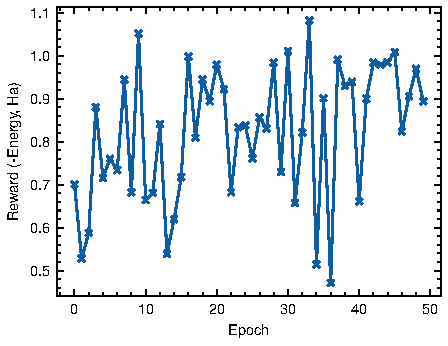
\includegraphics[width=\textwidth]{Figures/fig_h2_vac_init_search_rewards.pdf}
        \caption{Search rewards for the $H_2$ ansatz. We can see that for most of the 50 iterations, the reward for the best circuit sampled from the search tree stays over 0.7.}
        \label{fig:h2_search}
    \end{subfigure}
    ~ %add desired spacing between images, e. g. ~, \quad, \qquad, \hfill etc. 
      %(or a blank line to force the subfigure onto a new line)
    \begin{subfigure}[t]{0.48\textwidth}
        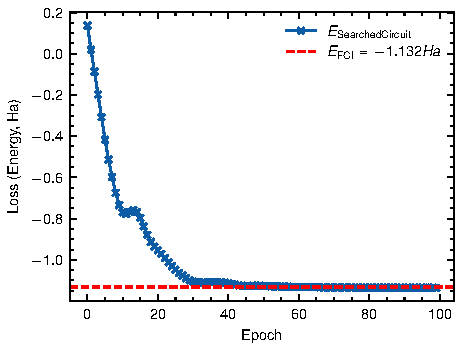
\includegraphics[width=\textwidth]{Figures/fig_h2_vac_init_fine_tune_loss.pdf}
        \caption{Fine-tune loss for the searched $H_2$ circuit. At the last iteration of optimization, the energy is around -1.1359 Ha, which is very close to the classically computed full configuration interaction result with PySCF \cite{Sun2018-nq, Sun2020-ej}, which is around -1.132 Ha and marked by the red horizontal dashed line.}
        \label{fig:h2_finetune}
    \end{subfigure}
    \caption{The search rewards and fine-tune loss for $H_2$ circuit. experiment.}\label{fig:h2_search_finetune}
\end{figure}

\begin{figure}[H]
  \centering
  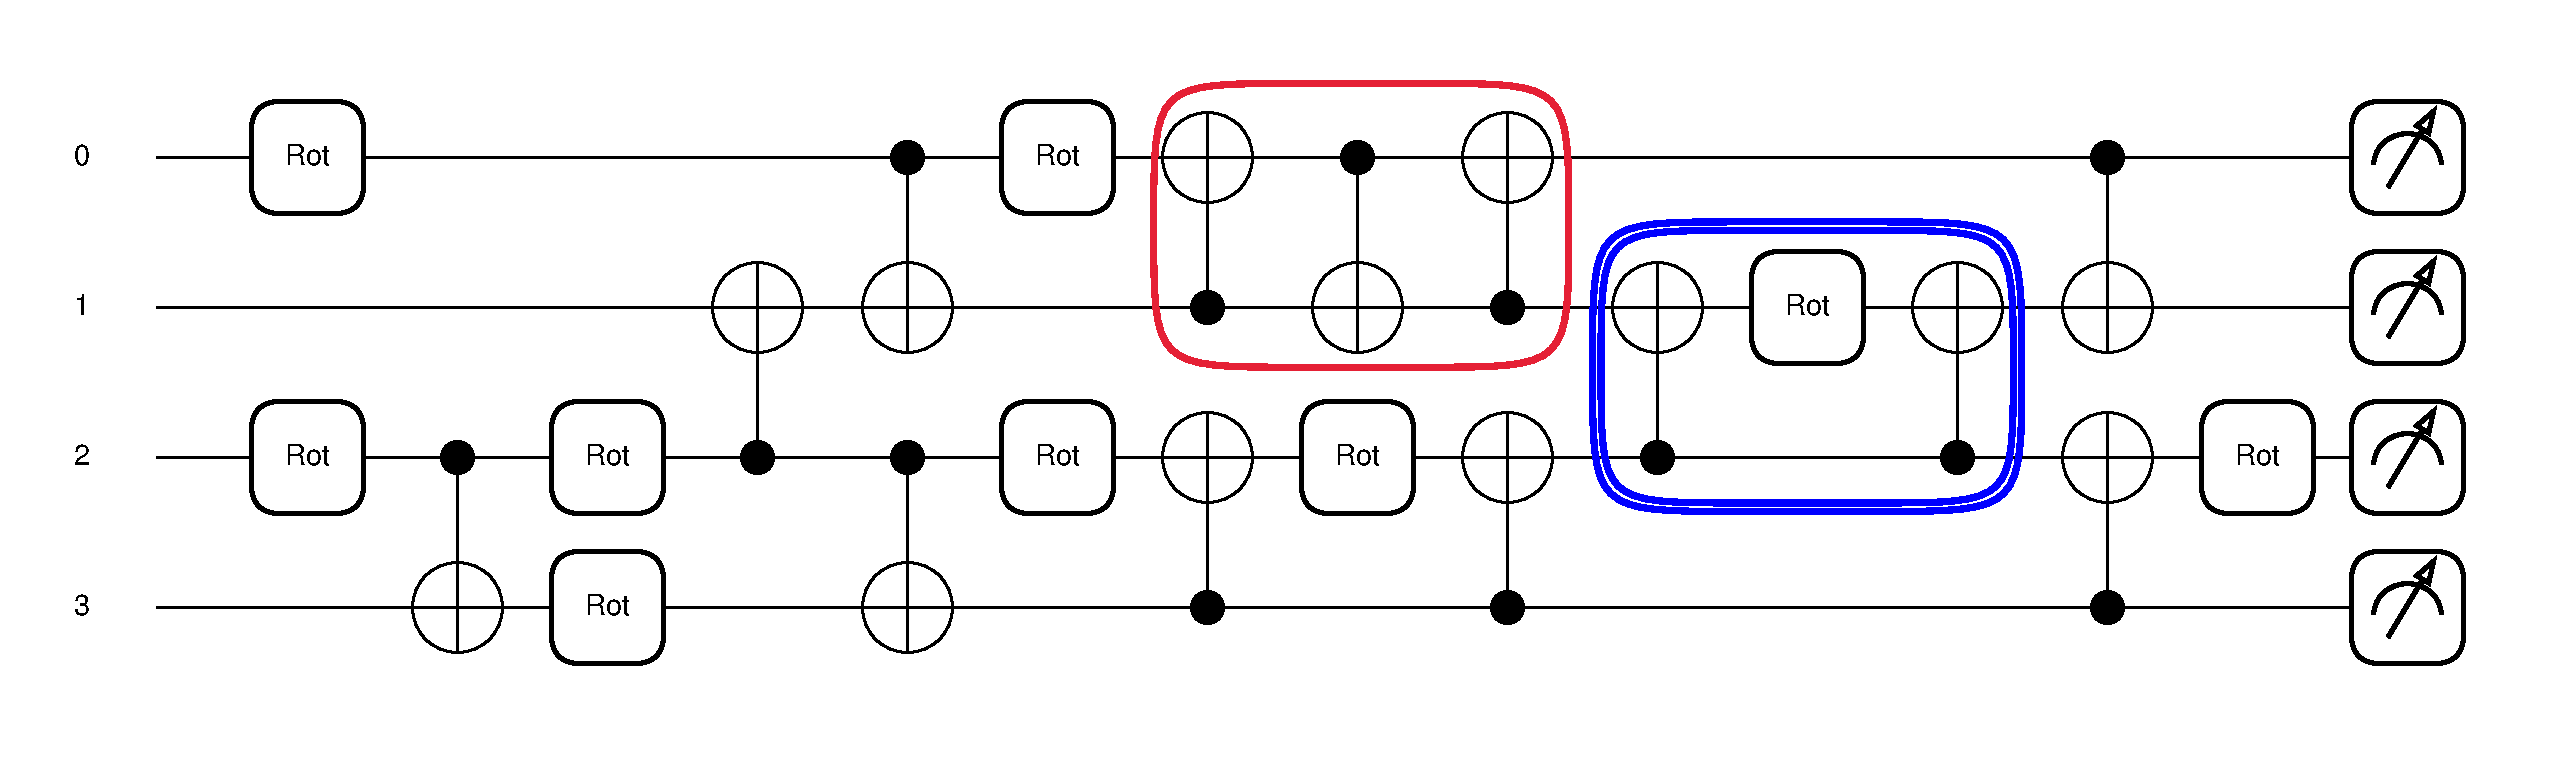
\includegraphics[width=0.95\textwidth]{Figures/fig_h2_vac_init_circ.pdf}
  \caption{The circuit for finding the ground energy of the $H_2$ molecule produced by the search algorithm. We can see that there are already familiar structures emerging: Red box: decomposition of the SWAP gate; Blue double-line box: Ising coupling-like circuit.}
  \label{fig:h2_circ}
\end{figure}



\paragraph{$LiH$ Results} The search reward when finding the suitable circuit structure for LiH is shown in Fig~\ref{fig:lih_search} and the training process for the circuit produced by the search algorithm is shown in Fig~\ref{fig:lih_finetune}. The ansatz is presented in Fig~\ref{fig:lih_circ}. The circuit produced by the search algorithm is simpler compared to the $H_2$ ansatz in Fig~\ref{fig:h2_circ}, indicating that the initial state may be very close to the ground energy state.
\begin{figure}[H]
    \centering
    \begin{subfigure}[t]{0.48\textwidth}
        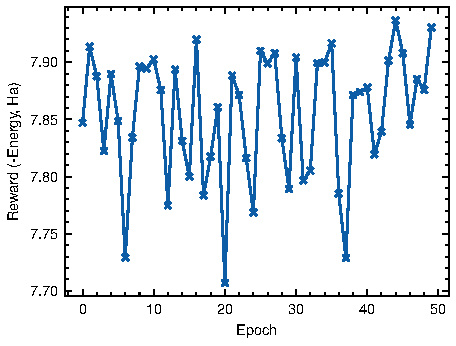
\includegraphics[width=\textwidth]{Figures/fig_lih_search_rewards.pdf}
        \caption{Search rewards for the $LiH$ ansatz. We can see that for most of the 50 iterations, the reward for the best circuit sampled from the search tree stays over 7.7.}
        \label{fig:lih_search}
    \end{subfigure}
    ~ %add desired spacing between images, e. g. ~, \quad, \qquad, \hfill etc. 
      %(or a blank line to force the subfigure onto a new line)
    \begin{subfigure}[t]{0.48\textwidth}
        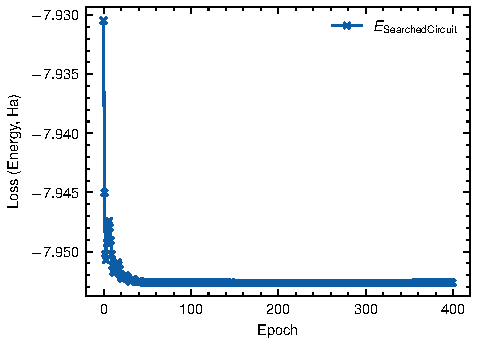
\includegraphics[width=\textwidth]{Figures/fig_lih_fine_tune_loss.pdf}
        \caption{Fine-tune loss for the searched $LiH$ circuit. At the last iteration of optimization, the energy is around -7.9526 Ha, very close to the classically computed full configuration interaction energy with PySCF \cite{Sun2018-nq, Sun2020-ej}, which is around -7.8885 Ha}
        \label{fig:lih_finetune}
    \end{subfigure}
    \caption{The search rewards and fine-tune loss for $LiH$ circuit. experiment.}\label{fig:lih_search_finetune}
\end{figure}

\begin{figure}[H]
  \centering
  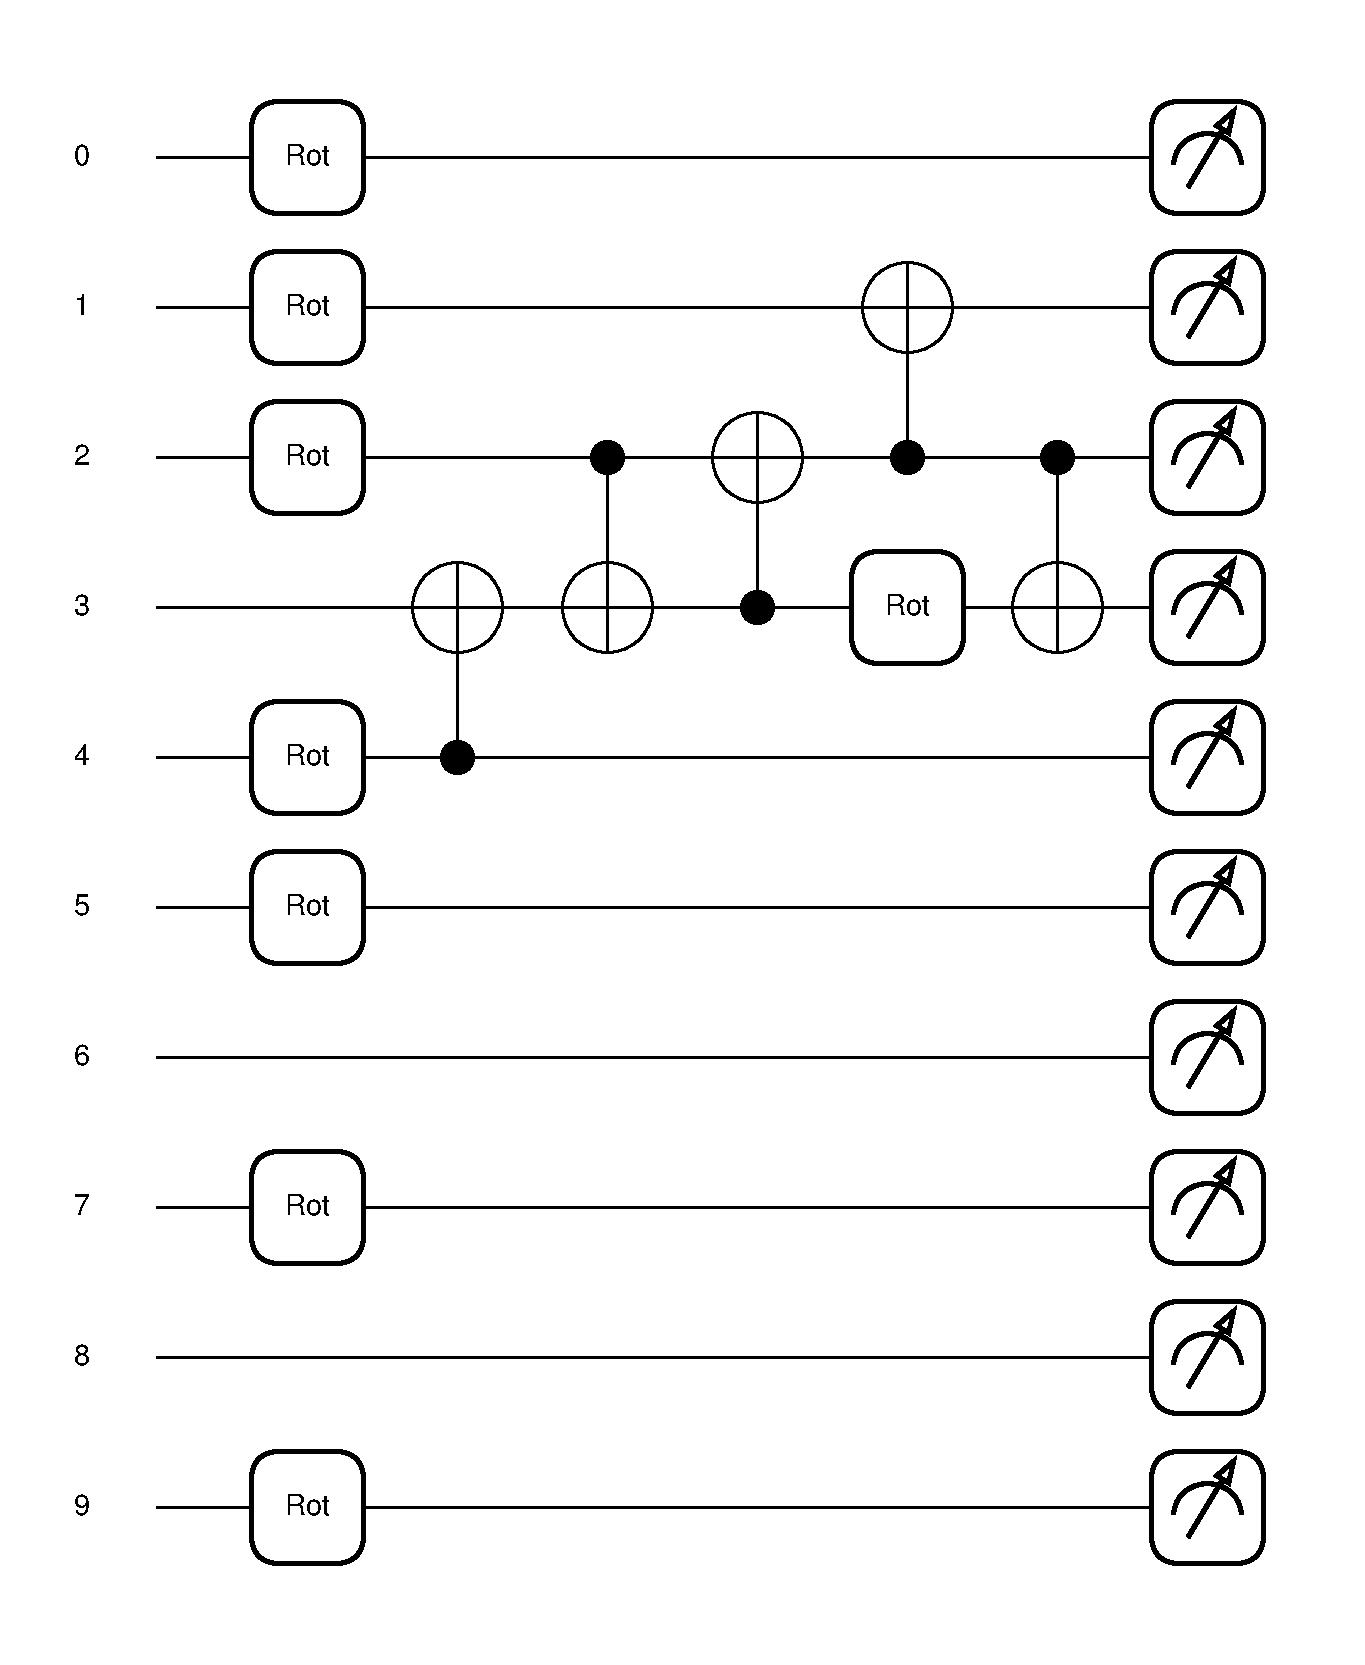
\includegraphics[width=0.6\textwidth]{Figures/fig_lih_circ.pdf}
  \caption{Circuit structure produced by the search algorithm for LiH. We can see that the structure of the circuit is quite simple, compared to the circuit for $H_2$ in Fig~\ref{fig:h2_circ}, indicating that the vacuum state $\ket{\psi_0} = \ket{0}^{\otimes 10}$ is already very close to the ground energy state.}
  \label{fig:lih_circ}
\end{figure}



\paragraph{$H_2 O$ Results} The search reward when finding the suitable circuit structure for $H_2 O$ is shown in Fig~\ref{fig:h2_search} and the training process for the circuit produced by the search algorithm is shown in Fig~\ref{fig:h2o_finetune}. The ansatz is presented in Fig~\ref{fig:h2o_circ}, which has 38 gates in total, including 10 local CNOT gates. Although there are still some familiar structures, such as the Ising coupling in the circuit, the heuristics behind most parts of the circuit are already unintuitive for human researchers.
\begin{figure}[H]
    \centering
    \begin{subfigure}[t]{0.48\textwidth}
        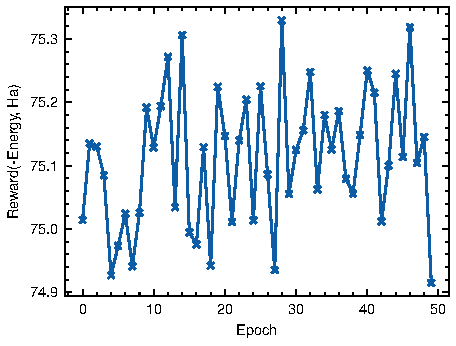
\includegraphics[width=\textwidth]{Figures/fig_H2O_search_rewards.pdf}
        \caption{Search rewards for the $H_2 O$ ansatz. We can see that for most of the 50 iterations, the reward for the best circuit sampled from the search tree stays over 74.9.}
        \label{fig:h2o_search}
    \end{subfigure}
    ~ %add desired spacing between images, e. g. ~, \quad, \qquad, \hfill etc. 
      %(or a blank line to force the subfigure onto a new line)
    \begin{subfigure}[t]{0.48\textwidth}
        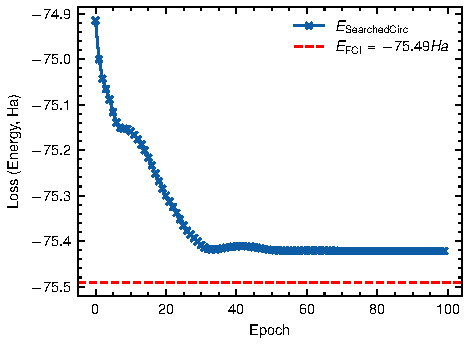
\includegraphics[width=\textwidth]{Figures/fig_H2O_fine_tune_loss.pdf}
        \caption{Fine-tune loss for the searched $H_2 O$ circuit. At the last iteration of optimization, the energy is around -75.4220  Ha, very close to the classically computed full configuration interaction energy with PySCF \cite{Sun2018-nq, Sun2020-ej}, which is around -75.4917  Ha}
        \label{fig:h2o_finetune}
    \end{subfigure}
    \caption{The search rewards and fine-tune loss for $LiH$ circuit.}\label{fig:h2o_search_finetune}
\end{figure}

\begin{figure}[H]
  \centering
  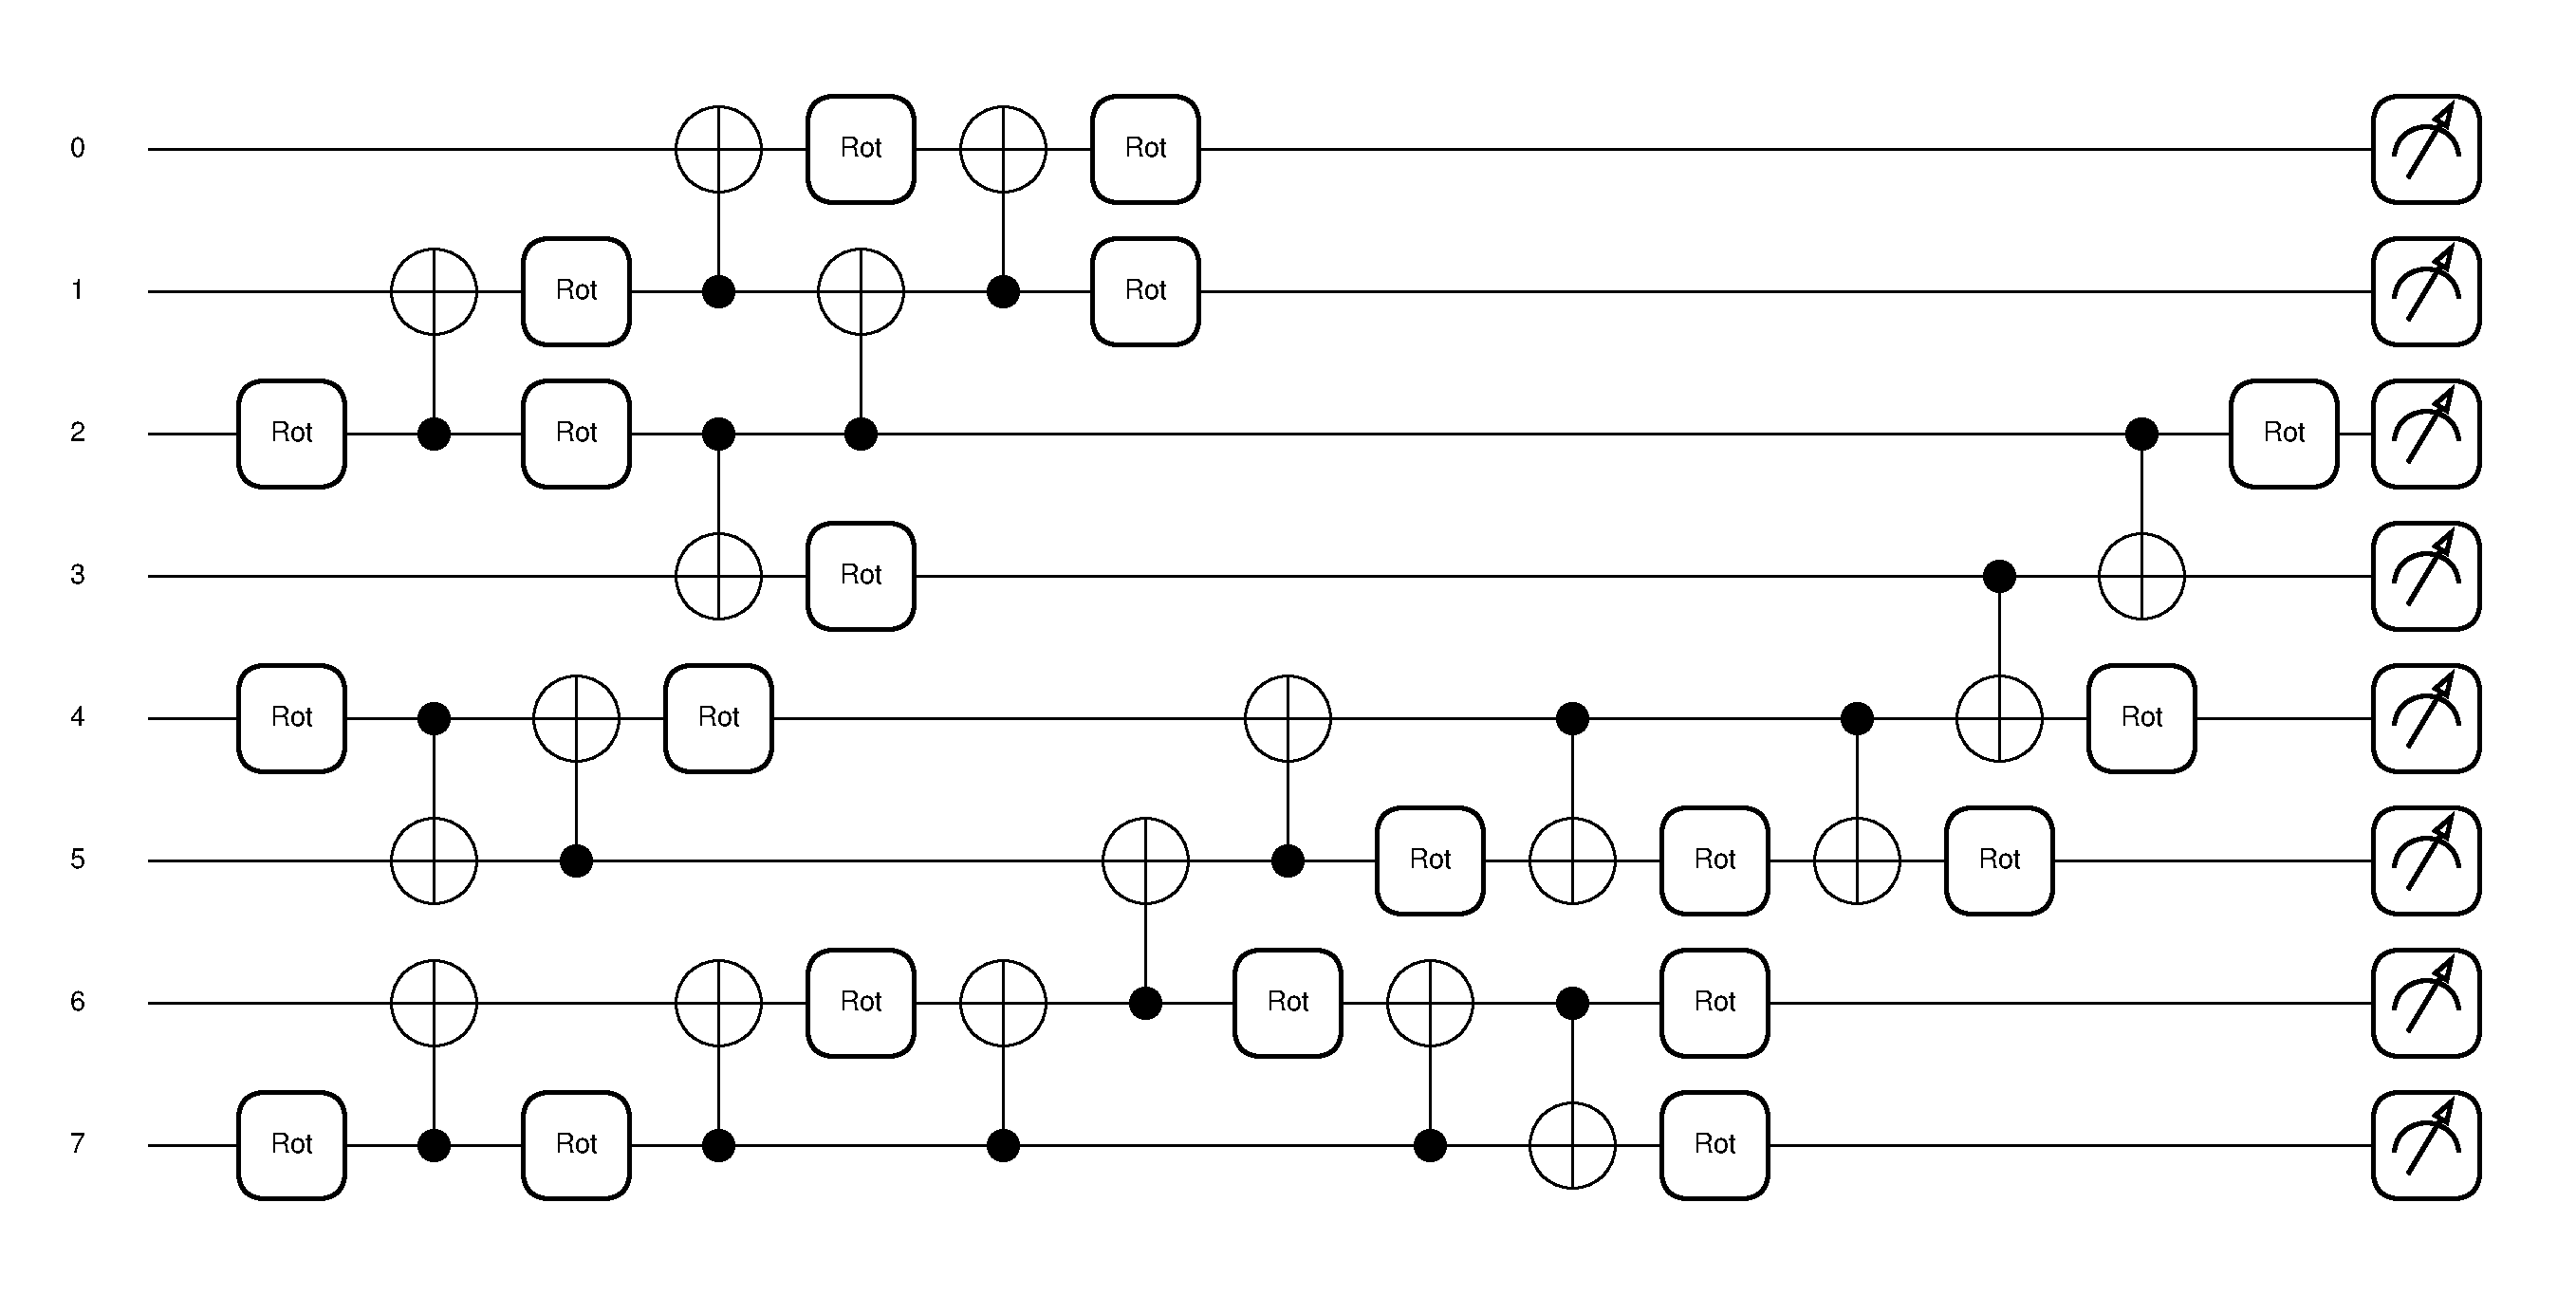
\includegraphics[width=0.9\textwidth]{Figures/fig_h2o_circ.pdf}
  \caption{Circuit for $H_2 O$ produced by the search algorithm.}
  \label{fig:h2o_circ}
\end{figure}


\subsection{Solving the \textsc{MaxCut} problem}
As a classic and well-known optimization problem, the \textsc{MaxCut} problem plays an important role in network science, circuit design, as well as physics \cite{Bharti2022-sw}. The objective of the \textsc{MaxCut} problem is to find a partition $z$ of vertices in a graph $G = (V, E)$ which maximizes the number of edges connecting the vertices in two disjoint sets $A$ and $B$:
\begin{equation}
    C(z) =\sum_{a=1}^m C_a(z)
\end{equation}
where $C_a(z) = 1$ if the $a^{th}$ edge connects one vortex in set $A$ and one vortex in set $B$, and $C_a(z) = 0$ otherwise. To perform the optimization on a quantum computer, we will need to transform the cost function into Ising formulation:
\begin{equation}
    H_C = -\sum_{(i, j)\in E} \frac{1}{2} (I - Z_i Z_j)w_{ij}
\end{equation}\label{qaoa_ham}
where $Z_i$ is the Pauli $Z$ operator on the $i^{th}$ qubit and $w_{ij}$ is the weight of edge $(i, j)\in E$ for weighted \textsc{MaxCut} problem. For unweighted problems, $w_{ij} = 1$. In this formulation, vertices are represented by qubits in computational bases. By finding the wave-function that minimizes the cost Hamiltonian $H_C$, we can find the solution that maximizes $C(z)$. Previously, the major components of the QAOA (quantum approximate optimization algorithm) ansatz are the cost Hamiltonian encoded by the cost unitary and the mixing Hamiltonians encoded by the mixing unitaries \cite{Farhi2014-ug}. Although this ansatz can find all the solutions in a equal superposition form, it is not always effective when the number of layers is small. Also, when the number of qubits (vertices) grows, the required number of layers and the number of shots during measurement to extract all of the solutions will also grow.

Since we have already had a Hamiltonian as our cost function in Sec.~\ref{h2}, we follow similar approach as quantum chemistry to find one of the solutions when the number of vertices is large.

\subsubsection{Experiment Settings}
\paragraph{Unweighted \textsc{MaxCut}}
\begin{figure}[H]
  \centering
  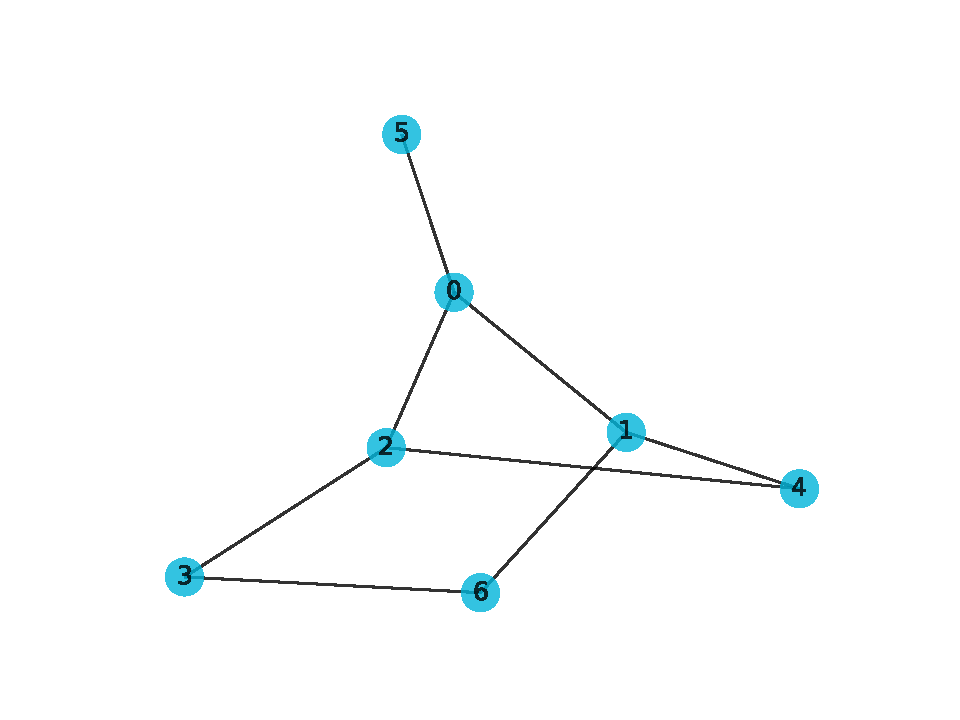
\includegraphics[width=0.8\textwidth]{Figures/fig_max_cut_large_7q.pdf}
  \caption{Problem graph for the unweighted \textsc{MaxCut} experiment}
  \label{fig:max_cut_prob}
\end{figure}
The problem graph for the unweighted \textsc{MaxCut} experiment is shown in Fig. \ref{fig:max_cut_prob}. This problem has six equally optimal solutions: 1001100, 0110010, 0111010, 1000101, 1001101 and 0110011, all have $C(z)=7$. The loss function is based on the expectation of the cost Hamiltonian $H_C$:
\begin{equation}
    L_{\textsc{MaxCut}} = (\bra{+})^{\otimes 7}U_{SearchedAnsatz}^{\dagger} H_C U_{SearchedAnsatz}   (\ket{+})^{\otimes 7}
\end{equation}
The reward function is simply the negative of the loss function:
\begin{equation}
    \mathcal{R}_{\textsc{MaxCut}} = -L_{\textsc{MaxCut}}
\end{equation}
We ran the search algorithm twice with the same basic settings, including the operation pool and the maximum number of layers. Since there is a random sampling process during the warm-up stage, the final solutions found by the algorithm are expected to be different. The operation pool consists of CNOT gates between every two qubits, the Placeholder and the single qubit rotation gate \cite{nielsen00}:
\begin{equation}
Rot(\phi, \theta, \omega)=R_Z(\omega) R_Y(\theta) R_Z(\phi)=\left[\begin{array}{cc}
e^{-i(\phi+\omega) / 2} \cos (\theta / 2) & -e^{i(\phi-\omega) / 2} \sin (\theta / 2) \\
e^{-i(\phi-\omega) / 2} \sin (\theta / 2) & e^{i(\phi+\omega) / 2} \cos (\theta / 2)
\end{array}\right]
\end{equation}
The size of the operation pool $c = \vert \mathcal{C} \vert = 28$, and the number of layers $p = 15$, leading to a search space of size $\vert \mathcal{S} \vert = 28^{15} \approx 5 \times10^{21}$. The `hard' restrictions on the maximum number of CNOT gates in a circuit, which is 7,  can help reduce the size of the search space.

\paragraph{Weighted \textsc{MaxCut}} For weighted \textsc{MaxCut}, we have a five-node graph, which is shown in Fig~\ref{fig:max_cut_weighted_prob}. The solution for this problem, 00011 (11100) is simpler than the unweighted version. The reward and loss function follow the same principle of the unweighted problem. The size of the operation pool $c = \mathcal{C} = 20$, and the number of layers $p = 10$, leading to a search space of size $\vert \mathcal{S} \vert = 20^{10} \approx 1.02\times 10^{13}$. The `hard' restriction on the maximum number of CNOTs in the circuit is 5.

\begin{figure}[H]
  \centering
  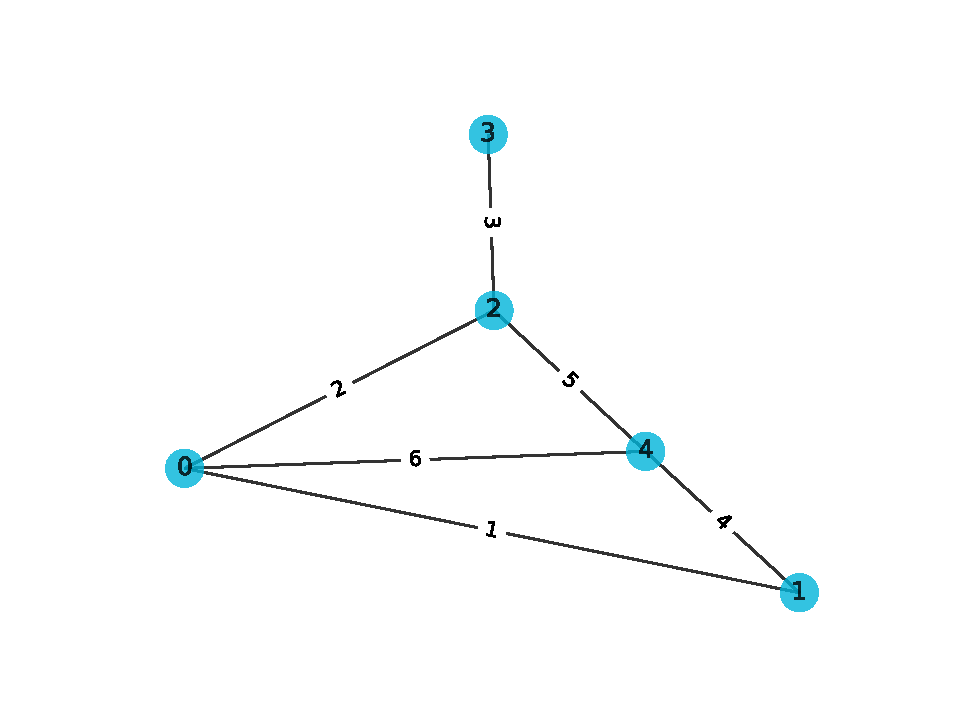
\includegraphics[width=0.8\textwidth]{Figures/fig_max_cut_weighted_5q.pdf}
  \caption{Problem graph for the weighted \textsc{MaxCut} experiment}
  \label{fig:max_cut_weighted_prob}
\end{figure}



\subsubsection{Results}
\paragraph{Unweighted \textsc{MaxCut}}
The two runs of the search algorithms gave us two circuits (Fig. \ref{fig:qaoa_7q_circ}), leading to two of the six optimal solutions (Fig. \ref{fig:qaoa_7q_solution}). The search rewards and fine-tune losses for both circuits are shown in Figure~\ref{fig:qaoa_7q_search_finetune_both}. During the search stage, since we already know the maximum reward it could reach is 7, and the reward can only be integers, we set the early-stopping limit to 6.5 to reduce the amount of time spent on searching, which means the algorithm will stop searching and proceed to fine-tuning the parameters in the circuit after the reward exceeds 6.5. In a real-world application, we could let the search algorithm run through all of the pre-set number of iterations and record the best circuit structure as well as the corresponding rewards at each iteration at the same time. Then after the search stage finishes, we can choose the best circuit (or top-k circuits) in the search history to fine-tune, increasing our chance to find the optimal solution.

\begin{figure}[H]
    \centering
    \begin{subfigure}[b]{0.48\textwidth}
        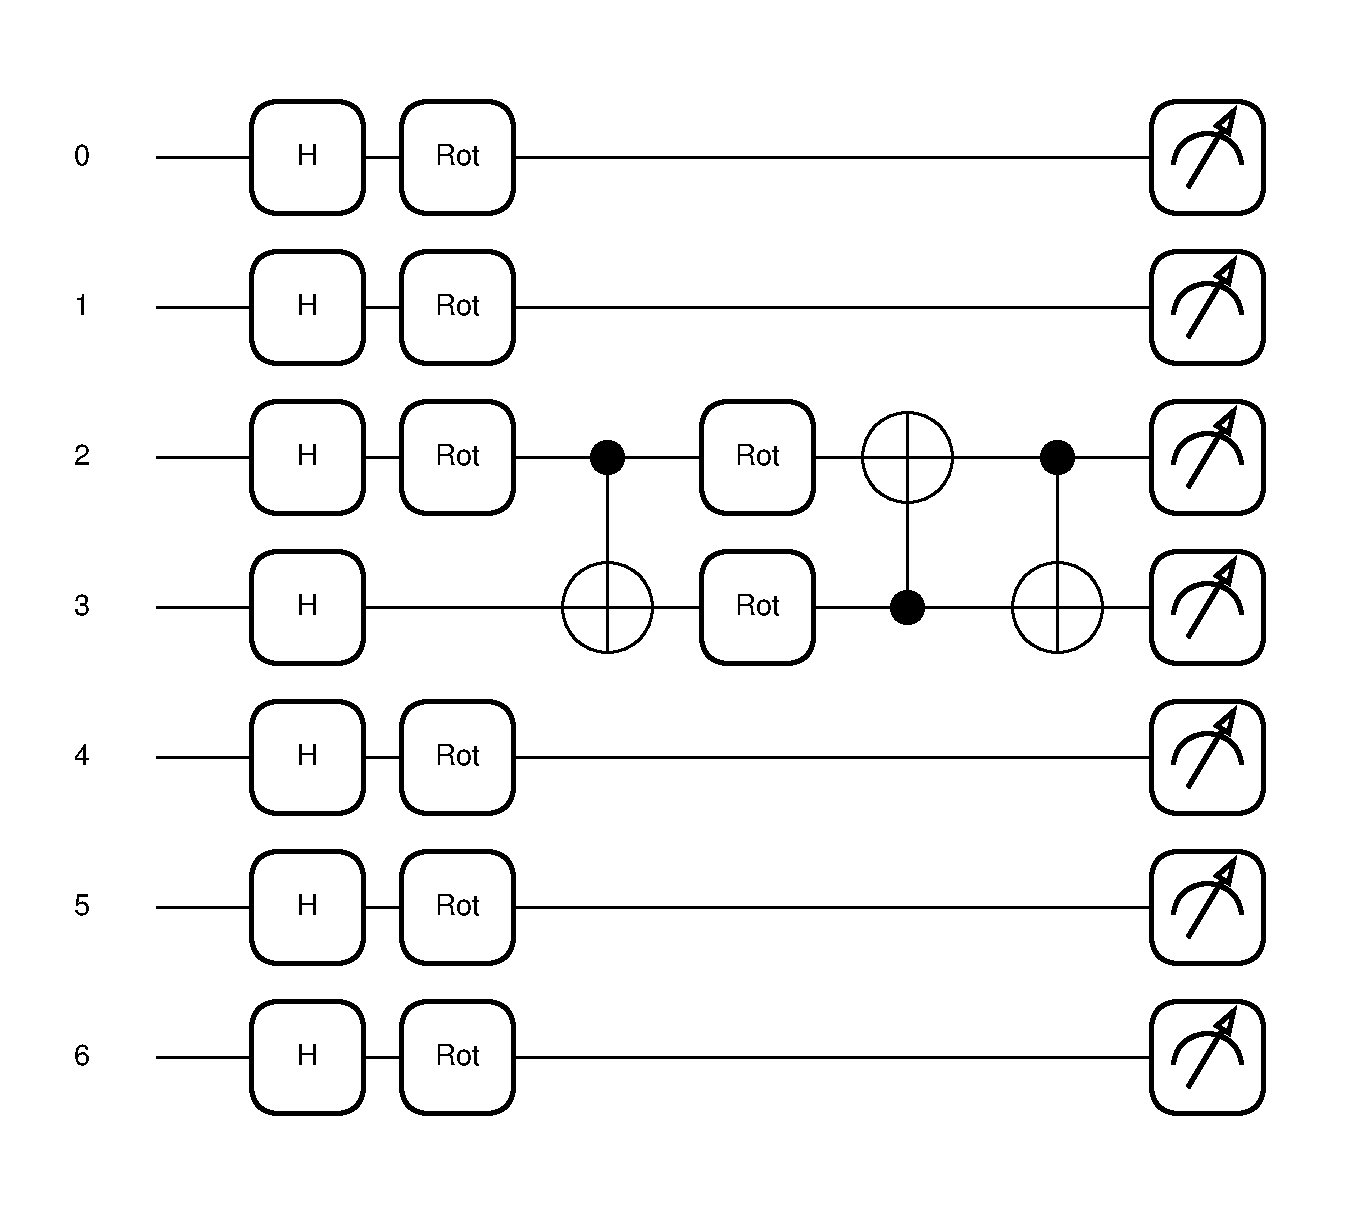
\includegraphics[width=0.75\textwidth]{Figures/fig_qaoa_circ_7q_1.pdf}
        \caption{}
        \label{fig:qaoa_7q_first_circ}
    \end{subfigure}
    ~ %add desired spacing between images, e. g. ~, \quad, \qquad, \hfill etc. 
      %(or a blank line to force the subfigure onto a new line)
    \begin{subfigure}[b]{0.48\textwidth}
        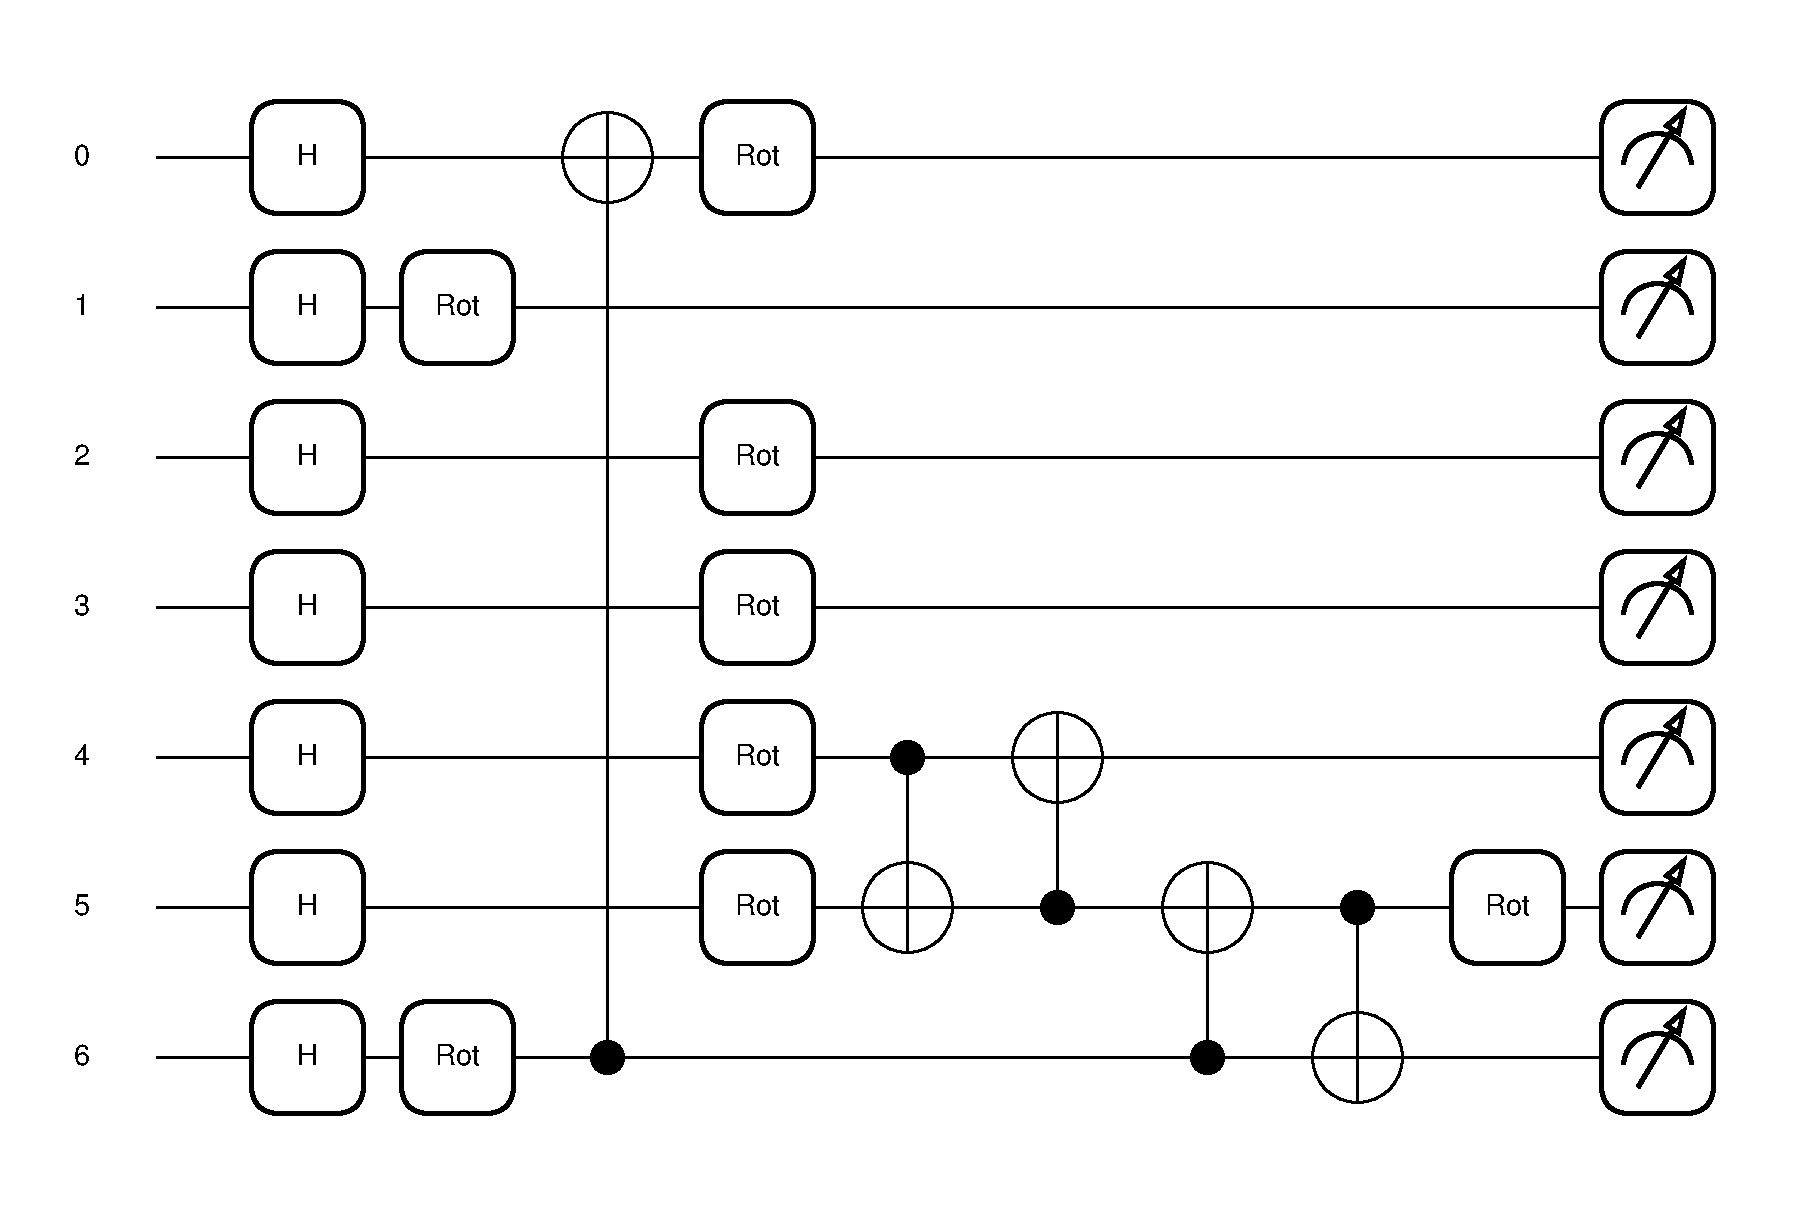
\includegraphics[width=\textwidth]{Figures/fig_qaoa_circ_7q_2.pdf}
        \caption{}
        \label{fig:qaoa_7q_second_circ}
    \end{subfigure}
    \caption{Two different circuits finding two different solutions of the \textsc{MaxCut} problem shown in Fig. \ref{fig:max_cut_prob}. Fig. \ref{fig:qaoa_7q_first_circ} gives the solution 0110010 (see Fig. \ref{fig:qaoa_7q_first_solution}) and Fig. \ref{fig:qaoa_7q_second_circ} gives the solution 0111010 (see Fig. \ref{fig:qaoa_7q_second_solution}).}\label{fig:qaoa_7q_circ}
\end{figure}

\begin{figure}[H]
    \centering
    \begin{subfigure}[b]{0.48\textwidth}
        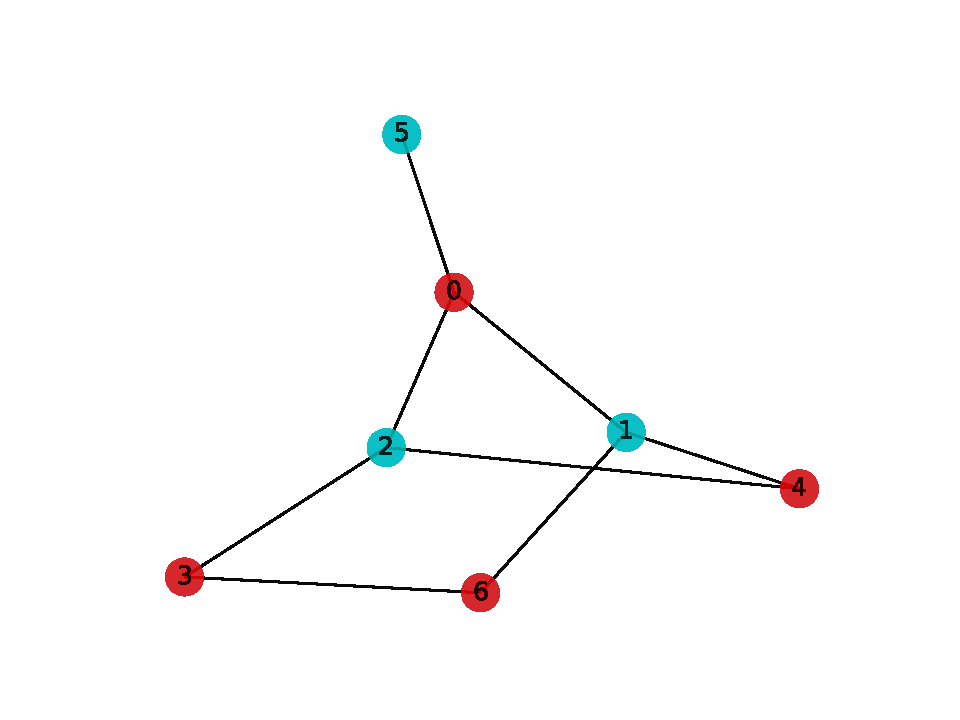
\includegraphics[width=\textwidth]{Figures/fig_maxcut_1_res_0110010.pdf}
        \caption{}
        \label{fig:qaoa_7q_first_solution}
    \end{subfigure}
    ~ %add desired spacing between images, e. g. ~, \quad, \qquad, \hfill etc. 
      %(or a blank line to force the subfigure onto a new line)
    \begin{subfigure}[b]{0.48\textwidth}
        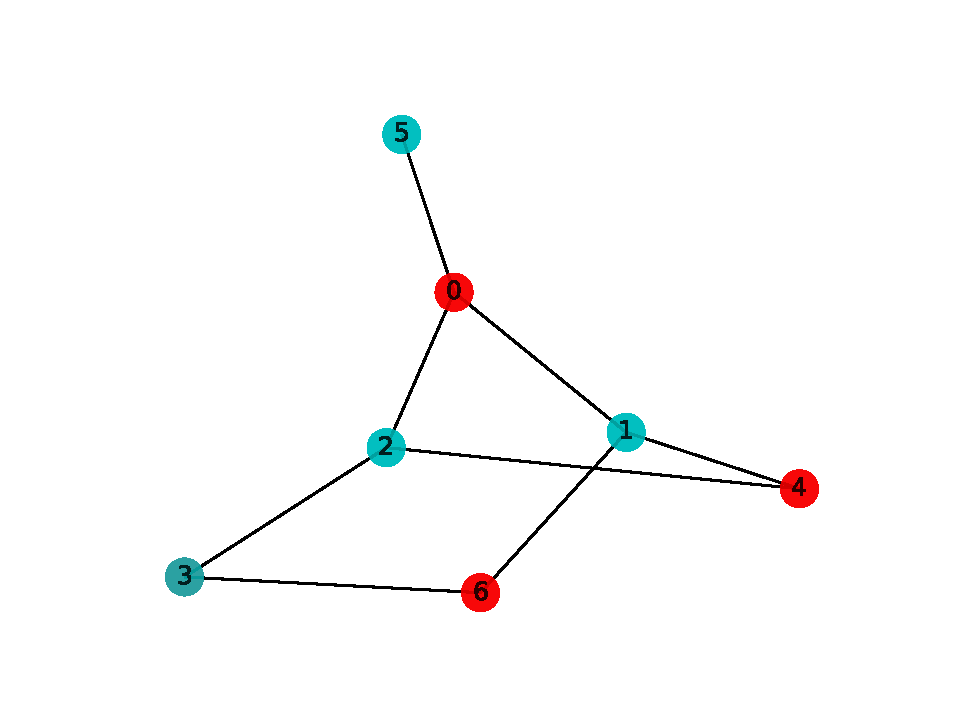
\includegraphics[width=\textwidth]{Figures/fig_maxcut_2_res_0111010.pdf}
        \caption{}
        \label{fig:qaoa_7q_second_solution}
    \end{subfigure}
    \caption{Two different optimal solutions found by the circuits in Fig. \ref{fig:qaoa_7q_first_circ} and Fig. \ref{fig:qaoa_7q_second_circ}, respectively.}\label{fig:qaoa_7q_solution}
\end{figure}


%\textcolor{red}{[Can we combine Figs.~(\ref{fig:qaoa_search_reward_1})-(\ref{fig:qaoa_finetune_2}) as four figures in a 2x2 grid or something similar?]}

\begin{figure}[H]
    \centering
    \begin{subfigure}[t]{0.48\textwidth}
        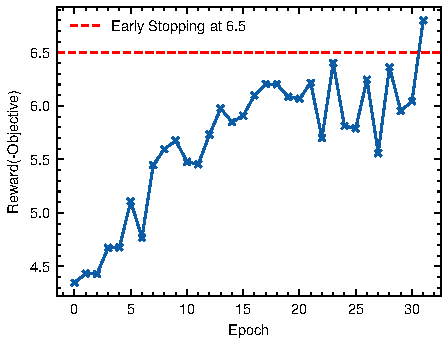
\includegraphics[width=0.95\textwidth]{Figures/fig_qaoa_7q_1_search_rewards.pdf}
        \caption{The change of rewards w.r.t. search iteration during the search for the ansatz (in Fig \ref{fig:qaoa_7q_first_circ}) that gives the solution 0110010 (Fig. \ref{fig:qaoa_7q_first_solution}). To reduce the amount of time for searching, we stopped the algorithm after the search reward exceeded 6.5.}
        \label{fig:qaoa_search_reward_1}
    \end{subfigure}
    ~
    \begin{subfigure}[t]{0.48\textwidth}
        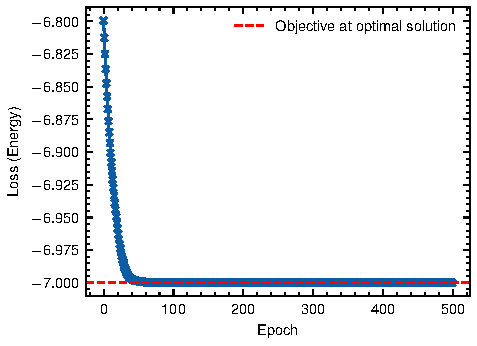
\includegraphics[width=\textwidth]{Figures/fig_qaoa_7q_1_fine_tune_loss.pdf}
        \caption{The change of loss w.r.t. optimization iteration during the fine-tune for the ansatz (in Fig \ref{fig:qaoa_7q_first_circ}) that gives the solution 0110010 (Fig. \ref{fig:qaoa_7q_first_solution}). We can see that the final loss is very close to -7, indicating that the circuit we found can produce an optimal solution.}
        \label{fig:qaoa_finetune_1}
    \end{subfigure}
    \hfill
    \begin{subfigure}[b]{0.48\textwidth}
        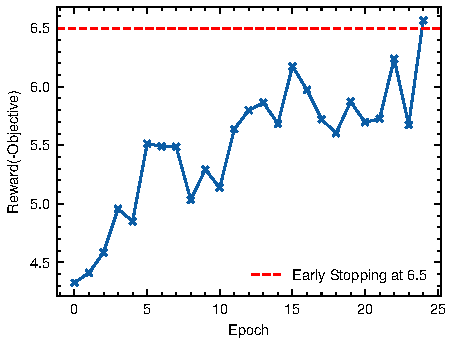
\includegraphics[width=0.99\textwidth]{Figures/fig_qaoa_7q_2_search_rewards.pdf}
        \caption{The change of rewards w.r.t. search iteration during the search for the ansatz (in Fig \ref{fig:qaoa_7q_second_circ}) that gives the solution 0111010 (Fig. \ref{fig:qaoa_7q_second_solution}). To reduce the amount of time for searching, we stopped the algorithm after the search reward exceeded 6.5.}
        \label{fig:qaoa_search_reward_2}
    \end{subfigure}
    ~
    \begin{subfigure}[b]{0.48\textwidth}
        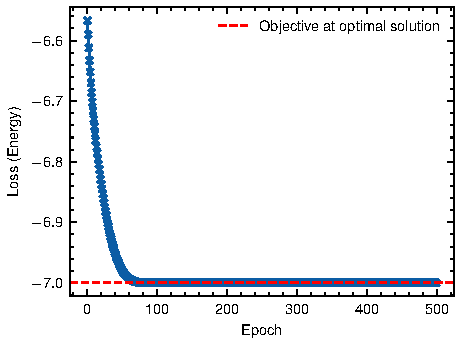
\includegraphics[width=\textwidth]{Figures/fig_qaoa_7q_2_fine_tune_loss.pdf}
        \caption{The change of loss w.r.t. optimization iteration during the fine-tune for the ansatz (in Fig \ref{fig:qaoa_7q_second_circ}) that gives the solution 0111010 (Fig. \ref{fig:qaoa_7q_second_solution}). We can see that the final loss is very close to -7, indicating that the circuit we found can produce an optimal solution.}
        \label{fig:qaoa_finetune_2}
    \end{subfigure}
    \caption{Search and fine-tune rewards for the circuits in Fig~\ref{fig:qaoa_7q_circ}. }\label{fig:qaoa_7q_search_finetune_both}
\end{figure}



\paragraph{Weighted \textsc{MaxCut}}
The search rewards and fine-tune losses for the weighted \textsc{MaxCut} problem are shown in Fig~\ref{fig:qaoa_5q_search_and_finetune}. We can see that the search converged quickly and the fine-tune loss is very close to -18, indicating that the circuit (see Fig~\ref{fig:qaoa_5q_circ}) produced by our search algorithm can indeed find an optimal solution (see Fig~\ref{fig:qaoa_5q_solution}).

\begin{figure}[H]
    \centering
    \begin{subfigure}[b]{0.46\textwidth}
        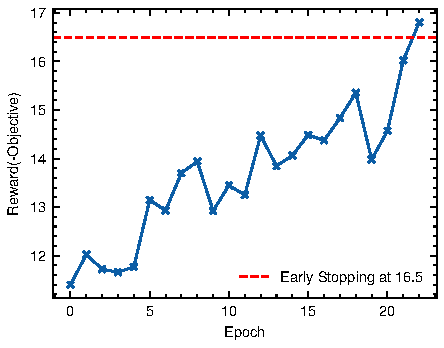
\includegraphics[width=\textwidth]{Figures/fig_qaoa_5q_1_search_rewards.pdf}
        \caption{Search rewards for the five-node weighted \textsc{MaxCut} problem}
        \label{fig:qaoa_5q_search}
    \end{subfigure}
    ~ %add desired spacing between images, e. g. ~, \quad, \qquad, \hfill etc. 
      %(or a blank line to force the subfigure onto a new line)
    \begin{subfigure}[b]{0.48\textwidth}
        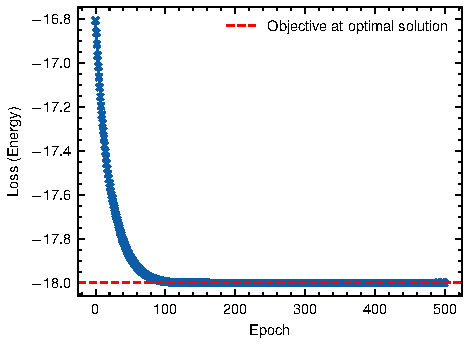
\includegraphics[width=\textwidth]{Figures/fig_qaoa_5q_1_fine_tune_loss.pdf}
        \caption{Fine-tune loss for the five-node weighted \textsc{MaxCut} problem}
        \label{fig:qaoa_5q_finetune}
    \end{subfigure}
    \caption{The search rewards and fine-tune losses of for the five-node \textsc{MaxCut} problem.}\label{fig:qaoa_5q_search_and_finetune}
\end{figure}


\begin{figure}[H]
    \centering
    \begin{subfigure}[b]{0.48\textwidth}
        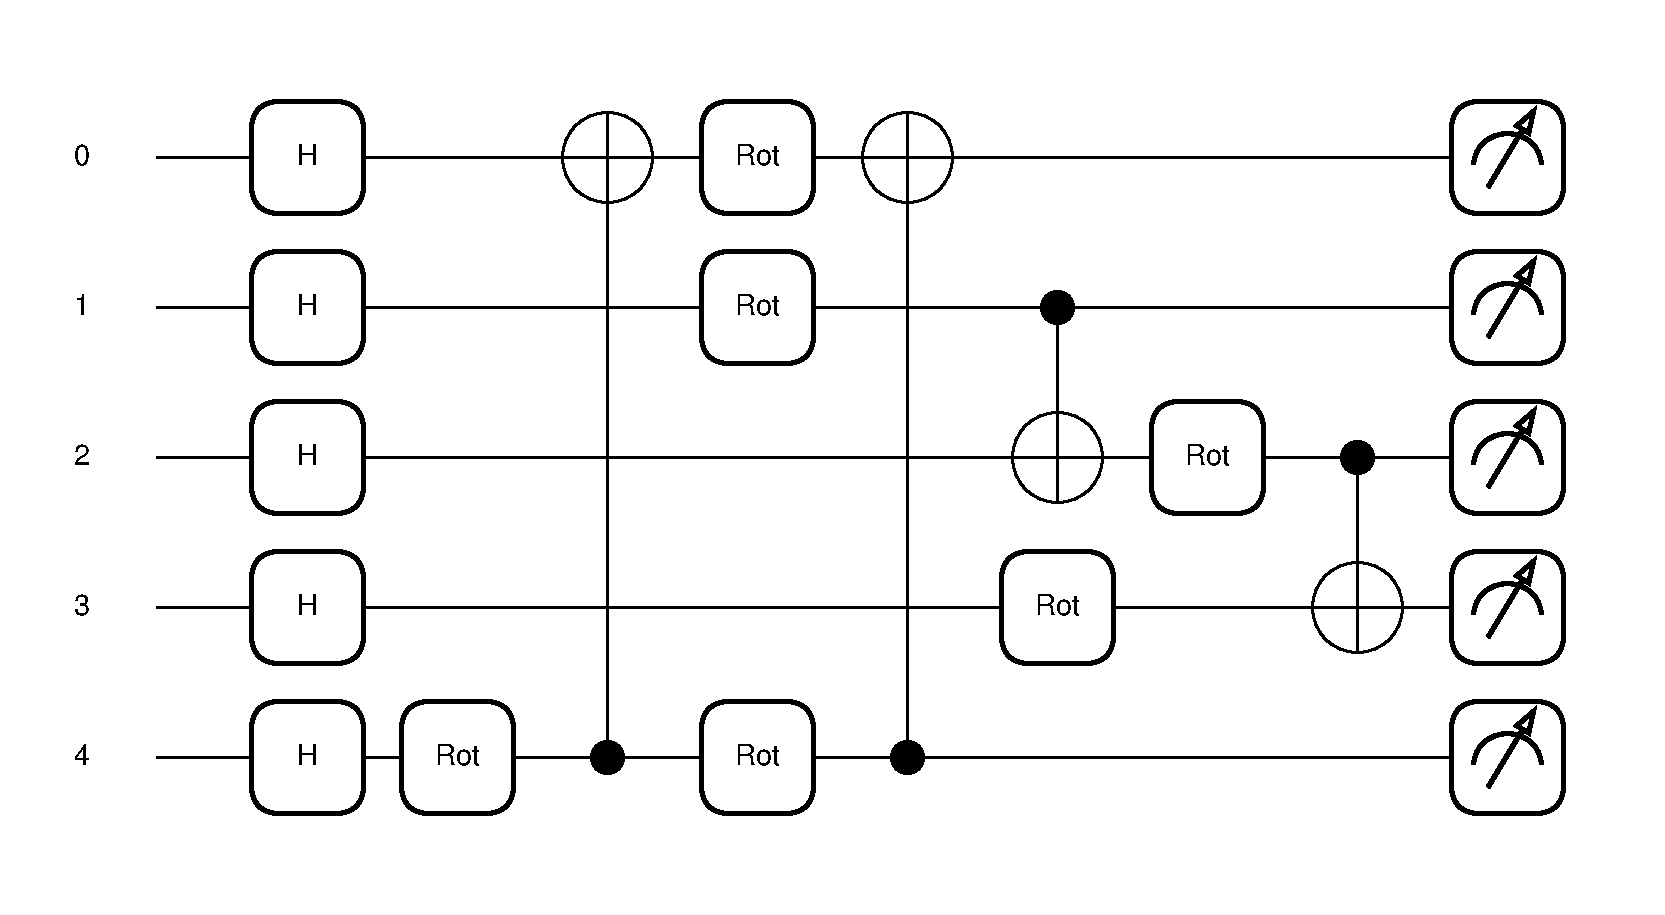
\includegraphics[width=\textwidth]{Figures/fig_qaoa_5q_circ.pdf}
        \caption{The searched circuit for the five-node weighted \textsc{MaxCut} problem}
        \label{fig:qaoa_5q_circ}
    \end{subfigure}
    ~ %add desired spacing between images, e. g. ~, \quad, \qquad, \hfill etc. 
      %(or a blank line to force the subfigure onto a new line)
    \begin{subfigure}[b]{0.46\textwidth}
        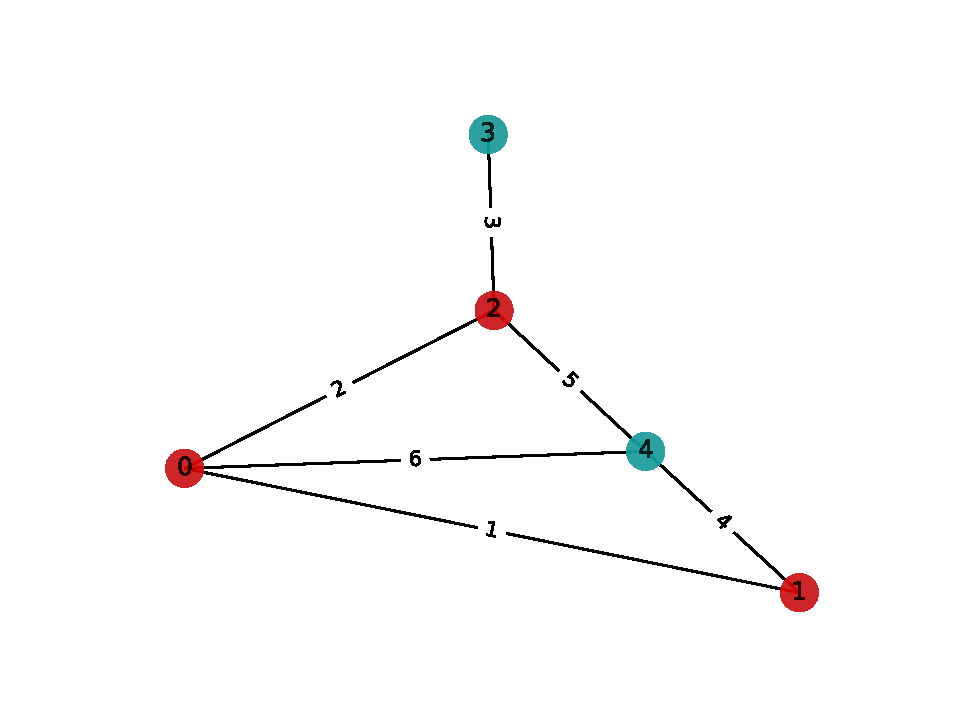
\includegraphics[width=\textwidth]{Figures/fig_maxcut_5q_res_00011.pdf}
        \caption{The solution sampled, which is 00011, from the circuit shown left.}
        \label{fig:qaoa_5q_solution}
    \end{subfigure}
    \caption{The searched circuit and sampled solution for the five-node \textsc{MaxCut} problem.}\label{fig:qaoa_5q_circ_and_solution}
\end{figure}





\section{Discussion}\label{discussion}
In this paper, we first formulated the circuit search problem as the tree structure. The sampled circuit can be represented as an arc (path from the root to a leaf) on the tree. We also introduced combinatorial multi-armed bandit and na\"ive assumption to model the selection of unitary operators for each layer in the circuit, and approximate the rewards of different unitaries with the reward of a fully constructed circuit. The search process is solved with Monte Carlo tree search (MCTS) algorithm. We demonstrated the effectiveness of our algorithmic framework with various examples, including finding the encoding circuit of the [[4,2,2]] quantum error detection code, developing the ans\"atz for variationally solving system of linear equations, searching the circuit for solving the ground state energy problem of different molecules, as well as circuits for solving optimization problems on a graph. To our understanding, we are the first to propose such a versatile framework for the automated discovery of quantum circuits with MCTS and combinatorial multi-armed bandits. Results showed that our framework can be applied to many different areas, especially those with problems that can be formulated as finding the ground state energy of a certain Hamiltonian.

From the experiments and results shown in the previous section, we can see that, by formulating quantum ansatz search as a tree-based search problem, one can easily impose various kinds of restrictions (`hard limits') on the circuit structure, leading to the pruning of the search tree and the search space. Also, by introducing Placeholders, one can explore smaller circuit sizes. Since current deep reinforcement learning algorithms struggle when the state space is large but the number of reward states is small. Compared to other research work in quantum ans\"atz search, including the differentiable quantum ans\"atz algorithm proposed in \cite{zhang2021differentiable}, and other QAS algorithms based on meta-learning \cite{chen2021quantum} or reinforcement learning \cite{kuo2021quantum}, which only investigate small-scale problems, like 3- or 4-qubit quantum Fourier transform in \cite{zhang2021differentiable}, 3-qubit classification task and 4-qubit $H_2$ ground state energy problem in \cite{du2020quantum}. A larger example can be seen in \cite{zhang2021neural}, which is a 6-qubit transversal Ising field model. In our research, we not only looked into 4-qubit systems like the $H_2$ molecule, but also larger systems like the $LiH$ and $H_2 O$ molecule as well as \textsc{MaxCut} on 7-node graphs. Our circuit depth is also often larger than the previous mentioned research. Since our operation pool consist of single-qubit gates on each qubit and CNOT gates either on neighbouring qubits or between every two qubits in the system, resulting a much larger size of operation pool compared to other research. With these two factors combined, our search space size is generally larger than other QAS research.
% By incorporating Monte Carlo tree search into the search of quantum circuits, as well as combinatorial multi-armed bandits, our algorithm can handle much larger search space compared to other QAS algorithms, which often look into problems with search space size with magnitude $10^3 \sim 10^7$\cite{chen2021quantum, du2020quantum, zhang2021differentiable, kuo2021quantum}.
%\textcolor{red}{[Are these the other pieces of work you're comparing your circuit to?]}

%\textcolor{red}{[You need to expand this discussion. Summarise what you found here, going through each case you considered (error detection, VQLS, QChem, max-cut). You want to write this first paragraph such that a reader will understand the significance and novelty of your work from reading this  discussion section alone. Also, you need to make stronger comparisons between the circuits you have found and the works you cite here, not just a general, overall claim of improvement. ]}

However, there are still several hyper-parameters that need to be tuned before the search algorithm can produce satisfying results, which leaves us space for improvement for the automation level of the algorithm. In the future, we would like to investigate the performance of our algorithm under noises, as well as improve the scalability of our algorithm by introducing parallelisation to the tree search algorithm when using a quantum simulator. We would also like to introduce more flexible value and/or policy functions into the algorithm.

\textcolor{red}{Overall, our work shows that MCTS method is a very efficient way to finding quantum circuits for a variety of problems and therefore it will be an important step towards widespread use of quantum variational circuits for many applications... }


%\paragraph{Note added:} During the preparation of this manuscript, we noticed that a relevant paper by Meng \textit{et.al} \cite{9566740mctsqas} also proposed applying Monte Carlo tree search to the problem of quantum ansatz search. However, their research didn't apply the nested Monte Carlo tree search and the na\"ive assumption of combinatorial multi-armed bandit, which will limit their performance when the tree branching factor is large.


\bibliographystyle{plain}
\typeout{} 
\bibliography{reference}



\end{document}
